\documentclass[10pt,twocolumn,letterpaper]{article}
\usepackage[left=0.58in,right=0.58in,top=0.68in,bottom=0.68in,columnsep=0.22in,headheight=11pt,headsep=8pt]{geometry}
\usepackage{mathptmx}
\usepackage{amsmath,amssymb}
\usepackage{graphicx}
\usepackage{booktabs}
\usepackage{tabularx}
\usepackage{array}
\usepackage{cite}
\usepackage{fancyhdr}
\usepackage{microtype}
\usepackage[hidelinks]{hyperref}
\usepackage{caption}
\IfFileExists{flushend.sty}{\usepackage{flushend}}{}

\flushbottom
\captionsetup{font=footnotesize,labelfont=bf,skip=3pt}
\setlength{\parskip}{0pt}
\setlength{\parindent}{1em}
\setlength{\textfloatsep}{7pt plus 2pt minus 2pt}
\setlength{\dbltextfloatsep}{7pt plus 2pt minus 2pt}
\setlength{\intextsep}{5pt plus 1pt minus 1pt}

\renewcommand{\topfraction}{0.92}
\renewcommand{\dbltopfraction}{0.92}
\renewcommand{\bottomfraction}{0.9}
\renewcommand{\textfraction}{0.07}
\renewcommand{\floatpagefraction}{0.85}
\renewcommand{\dblfloatpagefraction}{0.85}

\pagestyle{fancy}
\fancyhf{}
\fancyhead[L]{\scriptsize NUMA-OTS: NUMA-AWARE TASK SCHEDULING IN OPENMP}
\fancyhead[R]{\scriptsize ABU ZANOUNA AND SEYAM \hspace{0.5em} \thepage}
\renewcommand{\headrulewidth}{0pt}

\makeatletter
\renewcommand{\section}{\@startsection{section}{1}{\z@}%
  {-1.45ex \@plus -0.3ex \@minus -0.2ex}%
  {0.6ex \@plus 0.15ex}%
  {\normalfont\normalsize\centering\scshape}}
\renewcommand{\subsection}{\@startsection{subsection}{2}{\z@}%
  {-1.1ex \@plus -0.25ex \@minus -0.15ex}%
  {0.4ex \@plus 0.1ex}%
  {\normalfont\small\itshape}}
\renewcommand{\thesection}{\arabic{section}}
\renewcommand{\thesubsection}{\arabic{section}.\arabic{subsection}}
\makeatother

% ---------------------------------------------------------------------------
% Stage 1 Host & Stage 3 Valgrind Cachegrind macros (from env_versions.txt,
% host_lscpu.txt, and sniper_cache_energy.csv) + auto-generated DES metrics.
\newcommand{\hostcpu}{Intel Core i5-1035G1 (4 cores / 8 threads)}
\newcommand{\hostgcc}{GCC 15.2.0 (Ubuntu 15.2.0-16ubuntu1)}
\newcommand{\hostos}{Linux 6.18.58.1-microsoft-standard-WSL2 x86\_64}
\newcommand{\cgSpmvLthree}{SpMV simulated LL miss rate $94.20\% \to 21.13\%$ (global $6.21\% \to 1.32\%$, LL misses $-78.7\%$)}
\newcommand{\cgBfsLthree}{BFS simulated LL miss rate $89.46\% \to 33.14\%$ (global $10.14\% \to 2.53\%$, LL misses $-75.1\%$)}
\newcommand{\cgJoinPrLthree}{HashJoin simulated LL $95.86\% \to 30.22\%$ ($-76.3\%$); PageRank simulated LL $95.21\% \to 24.07\%$ ($-77.9\%$)}
\newcommand{\cgEnergySummary}{model-based micro-kernel energy estimates reduced by $32.2\%$--$50.6\%$: SpMV $2.710 \to 1.340$\,mJ, BFS $1.638 \to 0.824$\,mJ, HashJoin $3.644 \to 2.471$\,mJ, PageRank $2.653 \to 1.503$\,mJ}
% Auto-generated from live simulation CSV outputs by 08_populate_latex_metrics.py
\newcommand{\CaseStudyRows}{%
SpMV & 22.53 & 25.22 & 16.30 & 20.38 & 23.00 & 1.11$\times$ & 26.6\% & 64.83 / 2.34 \\
BFS & 5.09 & 5.13 & 4.46 & 4.93 & 5.75 & 1.03$\times$ & 29.0\% & 52.08 / 2.17 \\
HashJoin & 20.45 & 22.92 & 15.49 & 18.22 & 20.86 & 1.12$\times$ & 26.7\% & 64.88 / 2.34 \\
PageRank & 25.52 & 28.48 & 18.98 & 23.06 & 25.89 & 1.11$\times$ & 26.6\% & 64.95 / 2.34 \\
}

\newcommand{\MainSpeedupRows}{%
SpMV (2N) & 41.53$\pm$0.22 & 40.76 & 44.28 & 42.11 & \textbf{37.24} & 39.09 & 38.51$\pm$0.51 & 1.08$\times$ [1.07,1.08] & 6.4 & $1.12e-08$ & 1.08$\times$ (0.0\%) \\
SpMV (4N) & 22.53$\pm$0.12 & 20.38 & 16.30 & 23.00 & 17.54 & 14.74 & \textbf{14.62$\pm$0.23} & 1.54$\times$ [1.53,1.55] & 26.0 & $1.12e-08$ & 1.67$\times$ (8.2\%) \\
SpMV (8N) & 12.98$\pm$0.11 & 9.95 & 9.39 & 14.39 & \textbf{7.01} & 7.67 & 7.66$\pm$0.02 & 1.69$\times$ [1.69,1.70] & 53.0 & $1.12e-08$ & 1.97$\times$ (16.2\%) \\
\midrule
BFS (2N) & 8.33$\pm$0.08 & 8.44 & 8.78 & 8.58 & \textbf{8.21} & 8.40 & 8.27$\pm$0.03 & 1.01$\times$ [1.00,1.01] & 0.6 & $4.66e-03$ & 1.05$\times$ (4.7\%) \\
BFS (4N) & 5.09$\pm$0.07 & 4.93 & 4.46 & 5.75 & \textbf{4.29} & 4.71 & 4.69$\pm$0.02 & 1.09$\times$ [1.08,1.09] & 5.8 & $1.12e-08$ & 1.29$\times$ (18.9\%) \\
BFS (8N) & 3.60$\pm$0.04 & 3.22 & 3.09 & 4.30 & \textbf{3.08} & 3.62 & 3.59$\pm$0.05 & 1.00$\times$ [1.00,1.01] & 0.2 & $0.159$ (n.s.) & 1.50$\times$ (49.0\%) \\
\midrule
HashJoin (2N) & 37.75$\pm$0.18 & 40.58 & 40.19 & 38.53 & 36.91 & \textbf{36.74} & 37.05$\pm$0.08 & 1.02$\times$ [1.02,1.02] & 4.3 & $1.12e-08$ & 1.03$\times$ (0.7\%) \\
HashJoin (4N) & 20.45$\pm$0.16 & 18.22 & \textbf{15.49} & 20.86 & 16.15 & 15.64 & 15.51$\pm$0.15 & 1.32$\times$ [1.31,1.32] & 24.1 & $1.12e-08$ & 1.46$\times$ (10.9\%) \\
HashJoin (8N) & 11.81$\pm$0.10 & 8.98 & 8.60 & 12.88 & 7.85 & 7.29 & \textbf{7.28$\pm$0.11} & 1.62$\times$ [1.61,1.63] & 38.1 & $1.12e-08$ & 1.85$\times$ (14.1\%) \\
\midrule
PageRank (2N) & 47.32$\pm$0.22 & 49.66 & 50.11 & 47.80 & \textbf{43.95} & 44.69 & 44.10$\pm$0.95 & 1.07$\times$ [1.06,1.08] & 3.1 & $1.12e-08$ & 1.06$\times$ (1.0\%) \\
PageRank (4N) & 25.52$\pm$0.15 & 23.06 & 18.98 & 25.89 & 20.21 & 17.86 & \textbf{17.73$\pm$0.13} & 1.44$\times$ [1.44,1.44] & 47.9 & $1.12e-08$ & 1.57$\times$ (9.0\%) \\
PageRank (8N) & 14.64$\pm$0.12 & 11.35 & 10.73 & 15.98 & \textbf{8.31} & 8.70 & 8.68$\pm$0.05 & 1.69$\times$ [1.68,1.69] & 48.6 & $1.12e-08$ & 1.91$\times$ (13.2\%) \\
}

\newcommand{\AblationRows}{%
\texttt{Base} (central FIFO) & 1.00$\times$ (14.9\%) & 1.00$\times$ (17.5\%) & 1.00$\times$ (14.9\%) & 1.00$\times$ (14.8\%) \\
\texttt{Mem0} (\texttt{--membind=0}) & 0.90$\times$ (15.6\%) & 0.96$\times$ (20.2\%) & 0.90$\times$ (15.6\%) & 0.90$\times$ (15.6\%) \\
\texttt{Inter} (\texttt{--interleave=all}) & 1.38$\times$ (12.4\%) & 1.17$\times$ (13.1\%) & 1.37$\times$ (12.5\%) & 1.36$\times$ (12.4\%) \\
\texttt{ParFT} (static first-touch) & 1.30$\times$ (13.6\%) & 1.12$\times$ (14.5\%) & 1.31$\times$ (16.8\%) & 1.29$\times$ (13.6\%) \\
\texttt{AutoNUMA} (reactive faults) & 0.90$\times$ (16.1\%) & 0.84$\times$ (22.8\%) & 0.92$\times$ (15.8\%) & 0.92$\times$ (16.3\%) \\
M1 only (\texttt{depend} route) & 1.45$\times$ (40.9\%) & 1.14$\times$ (39.7\%) & 1.25$\times$ (40.1\%) & 1.31$\times$ (40.0\%) \\
M2 only (gated migration) & 0.94$\times$ (16.0\%) & 0.88$\times$ (22.7\%) & 0.95$\times$ (15.6\%) & 0.95$\times$ (16.0\%) \\
M3 only (3-tier SLIT queues) & 1.00$\times$ (14.9\%) & 0.98$\times$ (14.1\%) & 1.01$\times$ (16.1\%) & 1.00$\times$ (14.9\%) \\
M1 + M2 (no SLIT queues) & 1.28$\times$ (49.3\%) & 0.96$\times$ (40.7\%) & 1.25$\times$ (46.6\%) & 1.27$\times$ (48.9\%) \\
M1 + M3 (no migration) & 1.85$\times$ (72.7\%) & 1.17$\times$ (64.8\%) & 1.50$\times$ (72.7\%) & 1.76$\times$ (72.6\%) \\
M2 + M3 (no \texttt{depend} M1) & 0.91$\times$ (12.7\%) & 0.84$\times$ (14.1\%) & 0.93$\times$ (14.8\%) & 0.92$\times$ (12.6\%) \\
Ungated M2 ($\gamma{=}1.0, T_{\mathrm{cool}}{=}0$) & 1.69$\times$ (82.9\%) & 1.00$\times$ (66.4\%) & 1.62$\times$ (79.9\%) & 1.68$\times$ (82.8\%) \\
\textbf{Full NUMA-OTS (M1+M2+M3)} & \textbf{1.69$\times$ (82.9\%)} & \textbf{1.00$\times$ (66.4\%)} & \textbf{1.62$\times$ (80.0\%)} & \textbf{1.69$\times$ (82.9\%)} \\
}

\newcommand{\TelemetryEightNodeRows}{%
\texttt{Base} $\alpha_{\mathrm{loc}}$ & 14.9\% & 17.5\% & 14.9\% & 14.8\% \\
\textbf{Full OTS $\alpha_{\mathrm{loc}}$} & \textbf{82.9\%} & \textbf{66.4\%} & \textbf{80.0\%} & \textbf{82.9\%} \\
\texttt{Base} $T_{\mathrm{cont}}$ (ns) & 60.45 & 48.55 & 60.18 & 60.31 \\
\textbf{Full OTS $T_{\mathrm{cont}}$ (ns)} & \textbf{6.19} & \textbf{17.74} & \textbf{11.73} & \textbf{7.76} \\
Memory-stall fraction $f_{\mathrm{mem}}$ & 0.878 & 0.834 & 0.898 & 0.843 \\
Migrations / trial (Ungated $\to$ Full) & 472.5$\to$465.3 & 176.1$\to$156.9 & 384.0$\to$384.0 & 473.6$\to$468.3 \\
\textbf{6-Epoch re-migs (Ungated $\to$ Full)} & \textbf{8.9$\to$6.4} & \textbf{10.0$\to$0.0} & \textbf{5.4$\to$5.0} & \textbf{8.5$\to$6.0} \\
\textbf{Beneficial migration precision (Full)} & \textbf{96.4\%} & \textbf{83.8\%} & \textbf{96.0\%} & \textbf{96.5\%} \\
Critical-path mig.\ pause (ms, Full) & 1.417 & 0.599 & 1.114 & 1.418 \\
Total overhead (\% of makespan, Full) & 19.01\% & 16.88\% & 15.79\% & 16.84\% \\
Stage~1 DES LLC miss (\% Base $\to$ Full) & 43.6$\to$29.4 & 44.0$\to$42.3 & 43.0$\to$30.8 & 43.6$\to$29.5 \\
Dynamic energy (mJ, Base $\to$ Full) & 176.0$\to$114.7 & 35.6$\to$27.7 & 158.1$\to$104.9 & 202.5$\to$134.4 \\
Total energy (mJ, Base $\to$ Full) & 2044.6$\to$1218.0 & 554.4$\to$544.7 & 1858.3$\to$1152.4 & 2310.1$\to$1383.6 \\
}

\newcommand{\ControllerAccountingRows}{%
SpMV & 1024 & 1932 & 1300$\to$244 & 180 & 251.6k$\to$86.8k & 0.88$\to$0.48 & 88.0$\to$12.9 \\
BFS & 129 & 1542 & 1040$\to$418 & 280 & 99.2k$\to$48.0k & 0.34$\to$0.27 & 23.9$\to$15.7 \\
HashJoin & 768 & 1932 & 1293$\to$304 & 220 & 305.5k$\to$116.5k & 0.88$\to$0.65 & 88.0$\to$28.8 \\
PageRank & 1024 & 1932 & 1298$\to$242 & 200 & 278.6k$\to$96.4k & 0.88$\to$0.54 & 88.0$\to$17.0 \\
}

\newcommand{\SpdRangeAll}{$1.00\times$ to $1.69\times$}
\newcommand{\SpdRangeIterTwo}{$1.02\times$--$1.08\times$}
\newcommand{\SpdRangeIterFour}{$1.32\times$--$1.54\times$}
\newcommand{\SpdRangeIterEight}{$1.62\times$--$1.69\times$}
\newcommand{\MaxPHolmSig}{$p_{\mathrm{Holm}} \le 4.66e-03$}
\newcommand{\AlphaBaseEightRange}{$14.8\%$--$17.5\%$}
\newcommand{\AlphaOtsEightIterRange}{$80.0\%$--$82.9\%$}
\newcommand{\AlphaOtsEightAllRange}{$66.4\%$--$82.9\%$}
\newcommand{\AlphaOtsEightBfs}{$66.4\%$}
\newcommand{\TcontRedRange}{$63.5\%$--$89.8\%$}
\newcommand{\TcontBaseEightRange}{$48.55$--$60.45$\,ns}
\newcommand{\TcontOtsEightRange}{$6.19$--$17.74$\,ns}
\newcommand{\OvhdRangeAll}{$0.38\%$--$19.01\%$}
\newcommand{\OvhdRangeEight}{$15.79\%$--$19.01\%$}
\newcommand{\DynEnergyRedRange}{$22.0\%$--$34.8\%$}
\newcommand{\TotEnergyRedRange}{$1.7\%$--$40.4\%$}
\newcommand{\TotEnergyRedIterRange}{$38.0\%$--$40.4\%$}
\newcommand{\TotEnergyRedBfs}{$1.7\%$}
\newcommand{\DesLlcBaseRange}{$43.0\%$--$44.0\%$}
\newcommand{\DesLlcOtsRange}{$29.4\%$--$42.3\%$}
\newcommand{\CaseStudyAlphaRange}{$26.6\%$--$29.0\%$}
\newcommand{\CaseStudyTcontRange}{$52.08$--$64.95$\,ns}
\newcommand{\CaseStudyGammaRange}{$2.17$--$2.34$}
\newcommand{\CaseStudyBaseParftRange}{$1.03\times$--$1.12\times$}
\newcommand{\SpmvSpdAll}{$1.08\times$ (2N), $1.54\times$ (4N), and $1.69\times$ (8N)}
\newcommand{\PrSpdAll}{$1.07\times$ (2N), $1.44\times$ (4N), and $1.69\times$ (8N)}
\newcommand{\JoinSpdAll}{$1.02\times$ (2N), $1.32\times$ (4N), and $1.62\times$ (8N)}
\newcommand{\JoinInterFullRange}{$1.00\times$--$1.18\times$}
\newcommand{\BfsSpdAll}{$1.01\times$ (2N), $1.09\times$ (4N), and $1.00\times$ (8N)}
\newcommand{\BfsMthirteenAll}{$1.01\times$ (2N), $1.19\times$ (4N), and $1.17\times$ (8N)}
\newcommand{\BfsRfPredEight}{$1.50\times$}
\newcommand{\BfsRfErrEight}{$49.0\%$}
\newcommand{\IterRfErrRange}{$0.0\%$--$16.2\%$}
\newcommand{\MemZeroBeatRange}{$1.04\times$--$1.89\times$}
\newcommand{\InterBeatRange}{$0.86\times$--$1.24\times$}
\newcommand{\ParFtBeatRange}{$0.90\times$--$1.39\times$}
\newcommand{\AutoNumaBeatRange}{$1.04\times$--$1.88\times$}
\newcommand{\ReSixSummary}{SpMV $8.9 \to 6.4$, BFS $10.0 \to 0.0$, HashJoin $5.4 \to 5.0$, and PageRank $8.5 \to 6.0$ (beneficial migration precision $83.8\%$--$96.5\%$)}
\newcommand{\EpycEightSummary}{$1.72\times$ on SpMV, $0.98\times$ on BFS, $1.64\times$ on HashJoin, $1.71\times$ on PageRank}
\newcommand{\HookSummaryText}{intercepted $2,950$ \texttt{GOMP\_task} calls ($2,948$ with \texttt{depend} clauses, i.e., $99.93\%$), parsed $5,764$ locators with an $82.8\%$ PHHT hit ratio ($4,772$ hits, $992$ misses across $909$ per-task \texttt{move\_pages(2)} query syscalls; mean query batch $1.09$ pages/call), and submitted $216$ M2 page-migration requests across $9$ non-empty batches out of $27$ \texttt{GOMP\_taskwait} epochs (mean request batch $B=24.00$, max $49$ pages; $0$ kernel-confirmed cross-node moves on the single-node WSL2 host)}
\newcommand{\BatchHistSummary}{mean DES migration batch sizes on 8~domains are SpMV: $58.2$ (max 64), BFS: $39.2$ (max 64), HashJoin: $64.0$ (max 64), PageRank: $58.8$ (max 64)}
\newcommand{\GranSweepSummary}{8N BFS Full NUMA-OTS scales from $0.94\times$ at $19\,\mu$s to $1.01\times$ at $320\,\mu$s and $1.18\times$ at $2560\,\mu$s (vs.\ \texttt{M1+M3} at $1.17\times$), while 8N SpMV scales from $1.83\times$ to $2.02\times$}
\newcommand{\SensSweepSummary}{sweeping $\gamma \in [0.5, 3.0]$ on 8N SpMV yields $1.70\times$ at $\gamma=1.5$ vs.\ $1.71\times$ at $\gamma=3.0$; sweeping $T_{\mathrm{rem}}/T_{\mathrm{loc}} \in [1.25, 3.00]$ on 4N SpMV increases speedup monotonically from $1.35\times$ to $1.92\times$; sweeping misses/page/sweep $\in [2, 100]$ ($\times 10$ sweeps/phase) on 8N SpMV rises from $1.03\times$ at $2$ to a peak of $1.71\times$ at $20$ before all-controller saturation compresses speedup to $1.21\times$ at $100$; sweeping $f_{\mathrm{mem}} \in [0.21, 0.95]$ scales 8N SpMV speedup from $1.23\times$ to $1.72\times$; varying initial Node-0 page skew from $0\%$ to $100\%$ shifts 8N SpMV speedup from $1.31\times$ to $1.75\times$}

% ---------------------------------------------------------------------------

\begin{document}

\twocolumn[{%
\begin{center}
{\LARGE\bfseries NUMA-Aware Task Scheduling for Shared-Memory Parallel Applications Using OpenMP\par}
\vspace{0.5em}
{\large Khalil Ibrahim Abu Zanouna$^1$ and Mohammed Abdulsalam Seyam$^2$\par}
\vspace{0.2em}
{\small\itshape $^{1,2}$Computer Engineering Department, Faculty of Engineering, Islamic University of Gaza, Gaza, Palestine\par}
{\small\itshape E-mail: khalil500863335@gmail.com, moh.seyam0@gmail.com\par}
\vspace{0.6em}
\end{center}
\noindent{\small\textbf{\textit{Abstract}---Multi-socket servers partition physical memory into non-uniform memory access (NUMA) domains, yet mainstream OpenMP runtimes schedule explicit tasks without tracking where their data reside, inflating remote DRAM latency and memory-controller queueing. We present a simulation-based design and evaluation of NUMA-OTS, a NUMA-aware OpenMP task-scheduling architecture combining (M1) first-touch-aware task placement guided by \texttt{depend}-clause locators and a user-space Page-Home Hash Table (PHHT), (M2) access-frequency-based page migration gated by a batch-size-calibrated multi-domain cost-benefit model with hysteresis, cooldown, and a controller-congestion guard, and (M3) hierarchical node-local, socket-local, and global task queues with topology-ordered work stealing. Our evaluation distinguishes live OS/ABI mechanics from simulated multi-socket timing: (Stage~1) a live \texttt{LD\_PRELOAD} prototype for GNU \texttt{libgomp} implementing \texttt{GOMP\_task} locator parsing, PHHT metadata caching, and batched \texttt{move\_pages(2)} syscall submission, paired with a pure-C11 discrete-event simulator (DES) evaluating M1+M2+M3 (including full synchronous migration barrier pauses) across 2-, 4-, and 8-domain Intel Xeon and AMD EPYC topologies over 30 paired trials and 13 policies (including reactive AutoNUMA and component ablations); (Stage~2) optional 4-node QEMU virtual NUMA verification scripts; and (Stage~3) controlled single-hierarchy cache-reuse and model-based energy micro-benchmarks under Valgrind Cachegrind. Across SpMV, BFS, HashJoin, and PageRank, Full NUMA-OTS achieves simulated speedups of \SpdRangeAll{} (significant on 11 of 12 configurations, \MaxPHolmSig{}), raises 8-domain local DRAM access fractions from \AlphaBaseEightRange{} to \AlphaOtsEightAllRange{}, reduces controller queueing delay by \TcontRedRange{}, and outperforms reactive \texttt{AutoNUMA} by \AutoNumaBeatRange{}. Accounting for full synchronous migration pauses also shows that placement-only \texttt{M1+M3} outperforms synchronous \texttt{Full NUMA-OTS} on under-parallelized 8-domain BFS ($1.17\times$ vs.\ $1.00\times$, $p_{\mathrm{Holm}}=0.159$ n.s.) and on 8-domain SpMV/PageRank ($1.85\times$/$1.76\times$ vs.\ $1.69\times$/$1.69\times$), whereas synchronous M2 yields clear net gains on 4-domain iterative workloads and controller-bound 8-domain HashJoin ($1.62\times$ vs.\ $1.50\times$).}\par}
\vspace{0.3em}
\noindent{\small\textbf{\textit{Index Terms}---Data locality, discrete-event simulation, memory hierarchy, non-uniform memory access (NUMA), OpenMP, task scheduling, work stealing.}\par}
\vspace{0.7em}
}]

% ===========================================================================
\section{Introduction}

\subsection{NUMA Ubiquity in Modern Servers}
Contemporary multi-socket server processors partition physical memory across distributed locality domains to overcome the bus saturation of centralized shared-memory architectures \cite{ref1,ref2}. Within each NUMA domain, processor cores connect directly to integrated DRAM controllers, scaling aggregate memory bandwidth with socket count \cite{ref3,ref4}. When a core accesses cache lines hosted on a remote domain, coherence transactions traverse inter-socket interconnects, and uncoordinated thread and page placement can reduce performance by 30--60\% in memory-intensive NUMA workloads \cite{ref5,ref6}. Because modern multi-chiplet processors also expose multiple NUMA domains within a single socket under Sub-NUMA Clustering (SNC) or NUMA-per-Socket (NPS) modes \cite{ref7}, locality-aware scheduling is essential across mainstream server platforms.

\subsection{OpenMP's Locality Gap}
OpenMP 5.2 provides portable directives for explicit tasking (\texttt{task}, \texttt{taskloop}), sibling data-flow ordering (\texttt{depend}), and thread binding (\texttt{OMP\_PLACES}, \texttt{OMP\_PROC\_BIND}), while distinguishing thread affinity from per-task data affinity \cite{ref8}. In GNU \texttt{libgomp} \cite{ref9}, ready-task insertion uses \texttt{depend} locators solely for execution ordering without querying which NUMA domain hosts the referenced physical frames. While dynamic work stealing balances irregular task trees \cite{ref10}, unguided cross-socket steals separate computation from its data and inflate remote interconnect traffic \cite{ref11,ref12}.

Prior systems address distinct facets of this problem, including hierarchical thread-team bubbles in ForestGOMP \cite{ref13}, explicit region-footprint extensions in MIR \cite{ref14}, chip-level shared queues \cite{ref11}, and streaming data-flow compilers \cite{ref12}; Section~2 contrasts these designs. To study how \texttt{depend}-guided placement, cost-benefit-gated page migration, and topology-aligned queues interact under standard OpenMP tasking semantics, we investigate two quantitative research questions within a controlled simulation framework:
\begin{itemize}\setlength{\itemsep}{0pt}\setlength{\parskip}{0pt}\setlength{\topsep}{2pt}
\item \textit{RQ1}: Across what ranges of per-task duration ($\tau_{\mathrm{task}}$), memory intensity ($f_{\mathrm{mem}}$), and domain counts ($N_{\mathrm{dom}} \in \{2, 4, 8\}$) does combining residency-guided task routing with topology-aligned queues reduce remote DRAM accesses and execution time relative to NUMA-oblivious and reactive OS baselines?
\item \textit{RQ2}: Under what phase-length, batch-size ($B_{\mathrm{batch}}$), hysteresis ($\gamma$), cooldown ($T_{\mathrm{cool}}$), and controller-utilization thresholds does synchronous page migration yield net latency savings exceeding its critical-path transfer and TLB-shootdown pauses, and when should migration be disabled?
\end{itemize}

\subsection{Contributions: NUMA-OTS Design, Implementation, Evaluation}
We frame this work explicitly as a \textbf{simulation-based design and evaluation study} supported by a live \texttt{LD\_PRELOAD} ABI/syscall prototype and virtual-NUMA functional verification, rather than a bare-metal multi-socket runtime study. Our contributions are:
\begin{itemize}\setlength{\itemsep}{1pt}\setlength{\parskip}{0pt}\setlength{\topsep}{2pt}
\item \textbf{Design.} The NUMA-OTS architecture (Fig.~\ref{fig:arch}, Sec.~4): (M1) read-only \texttt{depend}-locator residency scoring backed by a 64-stripe Page-Home Hash Table (PHHT); (M2) batch-size-calibrated multi-domain cost-benefit page migration with a stabilized EMA demand predictor, hysteresis, cooldown, and a controller-congestion guard; and (M3) per-team three-tier topology-aligned queues with SLIT-ordered work stealing.
\item \textbf{Implementation.} A reproducible multi-level prototype and simulator suite (Sec.~5): (i)~a live \texttt{LD\_PRELOAD} shared library (\texttt{libnuma\_ots\_hook.so}) intercepting \texttt{GOMP\_task} and \texttt{GOMP\_taskwait} to verify GCC 13.2--15.2 \texttt{depend} parsing, PHHT metadata caching, M1 priority hinting, and \texttt{move\_pages(2)} syscall submission; (ii)~an 8-test OpenMP 5.2 and concurrency stress suite checked under ASan/UBSan; (iii)~a pure-C11 min-heap discrete-event simulator (DES) evaluating M1+M2+M3 scheduling with full synchronous migration pauses, closed-form M/M/1 controller accounting, per-domain LLC residency, and model-based static/dynamic energy accounting; (iv)~optional 4-node QEMU virtual-NUMA verification scripts; and (v)~controlled Valgrind Cachegrind micro-kernels.
\item \textbf{Evaluation.} Paired simulation experiments across 13 policies (including \texttt{numactl} equivalents, reactive \texttt{AutoNUMA}, and single/pairwise M1/M2/M3 ablations), 4 workloads (SpMV, BFS, HashJoin, PageRank), and 2, 4, and 8 NUMA domains (30 paired trials per configuration), plus systematic sensitivity sweeps over $\tau_{\mathrm{task}}$, $\gamma$, $T_{\mathrm{rem}}/T_{\mathrm{loc}}$, misses/page, $f_{\mathrm{mem}}$, and initial page skew (Sec.~6), showing both positive and negative migration regimes.
\end{itemize}

% ===========================================================================
\section{Background}

\subsection{NUMA Architecture Fundamentals}
Classical uniform-memory-access (UMA) multiprocessors route memory requests over a shared bus or crossbar \cite{ref15}. As core counts scale, centralized controllers saturate; ccNUMA servers distribute physical memory across $N_{\mathrm{dom}}$ locality domains, configured either as one domain per socket or as multiple intra-socket domains under SNC/NPS \cite{ref7}. Cache-sharing boundaries (L2/LLC slices) need not align one-to-one with NUMA domains \cite{ref16}.

Under a first-order mean-value approximation incorporating an effective memory-level parallelism overlap factor $\eta_{\mathrm{MLP}} \in (0, 1]$, the effective service time contributed per LLC miss that reaches DRAM is
\begin{equation}
E[T_{\mathrm{mem}} \mid \text{DRAM miss}] = \eta_{\mathrm{MLP}}\Bigl[\alpha_{\mathrm{loc}}\, T_{\mathrm{loc}} + (1 - \alpha_{\mathrm{loc}})\,\overline{T}_{\mathrm{rem}} + T_{\mathrm{cont}}(\lambda)\Bigr],
\label{eq:latency}
\end{equation}
where $\alpha_{\mathrm{loc}} \in [0,1]$ is the local DRAM hit fraction, $T_{\mathrm{loc}}$ the unloaded local latency, $\overline{T}_{\mathrm{rem}} > T_{\mathrm{loc}}$ the distance-weighted unloaded remote latency, and $T_{\mathrm{cont}}(\lambda) \ge 0$ the controller queueing delay under request-rate vector $\lambda$. Because ACPI SLIT tables (Sec.~5.2.17 of \cite{ref17}) report normalized relative distances rather than nanoseconds, latency matrices $L(d,x)$ must be calibrated from pointer-chasing benchmarks; prior studies \cite{ref18} show that $T_{\mathrm{cont}}(\lambda)$ can dominate stall time when hot pages saturate one controller.

Under the Roofline model \cite{ref19}, for a kernel whose ideal all-local DRAM stall time (already scaled by $\eta_{\mathrm{MLP}}$) forms a fraction $f_{\mathrm{mem}} \in (0,1]$ of its ideal all-local execution time, relative runtime scales with the latency inflation factor $\Gamma = E[T_{\mathrm{mem}}]/(\eta_{\mathrm{MLP}} T_{\mathrm{loc}})$ as
\begin{equation}
T_{\mathrm{rel}} \approx (1 - f_{\mathrm{mem}}) + f_{\mathrm{mem}}\,\Gamma .
\label{eq:roofline}
\end{equation}
Notice that $\eta_{\mathrm{MLP}}$ cancels in $\Gamma$ while shaping $f_{\mathrm{mem}}$. We use Eqs.~(\ref{eq:latency})--(\ref{eq:roofline}) strictly as an \emph{internal analytical consistency check} of the simulator (Sec.~6.4), not as external hardware validation.

\subsection{OpenMP Tasking Model (\texttt{task}, \texttt{taskloop}, \texttt{depend})}
An OpenMP \texttt{task} packages a code block and its data environment for deferred execution by any thread of the binding team; \texttt{taskwait}, \texttt{taskgroup}, and barriers provide completion synchronization. \texttt{taskloop} partitions a loop into tasks by \texttt{grainsize} or \texttt{num\_tasks}. The \texttt{depend} clause (\texttt{in}, \texttt{out}, \texttt{inout}, \texttt{mutexinoutset}, \texttt{inoutset}) orders sibling tasks by the storage locations they name. OpenMP 5.2 specifies tasking and the task \texttt{affinity} clause in Secs.~12.5--12.6 (specifically Sec.~12.5.1), task scheduling constraints (TSCs) in Sec.~12.9, dependences in Sec.~15.9.5, and thread-binding controls (\texttt{OMP\_PLACES}, \texttt{OMP\_PROC\_BIND}) in Secs.~21.1.6--21.1.7 \cite{ref8}. Thread binding (\texttt{OMP\_PLACES}, \texttt{OMP\_PROC\_BIND}) pins OS threads to cores, whereas the OpenMP 5.0 \texttt{affinity} clause provides per-task data hints that remain a no-op stub in GNU \texttt{libgomp} \cite{ref9}. Furthermore, OpenMP 5.2 does \emph{not} permit \texttt{depend} on \texttt{taskloop} (deferred to OpenMP 6.0 \texttt{task\_iteration}).

In GNU \texttt{libgomp} (\texttt{libgomp.h}, \texttt{task.c}) \cite{ref9}, tasks traverse team-level (\texttt{team->task\_queue} under \texttt{team->task\_lock}), parent-level (\texttt{children\_queue}, \texttt{depend\_hash}), and \texttt{taskgroup\_queue} scopes. When GCC emits \texttt{GOMP\_task} for array sections (\texttt{a[0:N]}), the ABI passes only base addresses, not byte extents \cite{ref20}. NUMA-OTS therefore treats \texttt{depend} locators strictly as approximate base-page locality hints.

\subsection{Existing NUMA-Aware Approaches: \texttt{numactl}, \texttt{likwid}, \texttt{hwloc}}
\texttt{numactl}/\texttt{libnuma} \cite{ref21} applies static, process-wide memory policies (\texttt{--membind}, \texttt{--interleave}) and exposes \texttt{move\_pages(2)}; it is task-blind. LIKWID (\texttt{likwid-pin}) \cite{ref22} pins threads and reads hardware performance counters without placing tasks or migrating pages. \texttt{hwloc} \cite{ref16} discovers hardware topology (ACPI SLIT, caches, cores) and provides binding primitives, serving as a topology substrate for runtimes.

\subsection{Related Work in Thread and Data Placement}
Table~\ref{tab:comparison} contrasts NUMA-OTS with OS kernel policies (Carrefour \cite{ref6}, kMAF \cite{ref23}, Linux AutoNUMA \cite{ref7}) and task/data-flow runtimes (ForestGOMP \cite{ref13}, Olivier et al. \cite{ref11}, OpenStream \cite{ref12}, and MIR \cite{ref14}). Kernel policies such as AutoNUMA react to minor page faults at OS-thread granularity without visibility into user-space OpenMP task DAGs. Task runtimes such as StarPU, OmpSs-2/Nanos6, and MIR offer locality-aware descriptors, but require non-standard runtime APIs or compiler extensions \cite{ref12,ref14} or omit cost-benefit-gated page migration \cite{ref11,ref14}. NUMA-OTS derives locality from standard OpenMP \texttt{depend} locators and couples task routing with batch-calibrated page migration.

\begin{table*}[!t]
\centering
\caption{Comparison of System-Level NUMA Utilities, OS/Runtime Policies, and the Proposed NUMA-OTS Design}
\label{tab:comparison}
\resizebox{\textwidth}{!}{%
\begin{tabular}{@{}l p{2.3cm} p{2.6cm} p{3.0cm} p{3.6cm} p{3.3cm}@{}}
\toprule
\textbf{System / Tool} & \textbf{Control Scope} & \textbf{Locality Signal} & \textbf{Queue \& Steal Design} & \textbf{Page Migration Policy} & \textbf{Implementation / Compatibility} \\
\midrule
Carrefour \cite{ref6} & OS kernel threads \& pages & Hardware PMU instruction sampling & OS thread clustering (no task-DAG visibility) & Reactive kernel replication, interleaving, \& migration & Kernel patch (no user task-DAG API) \\
Linux AutoNUMA \cite{ref7} & OS kernel threads \& pages & Periodic \texttt{PROT\_NONE} hint faults & OS scheduler balancing & Reactive fault-driven page migration & Stock Linux kernel (task-blind) \\
Olivier et al. \cite{ref11} & Unstructured \texttt{omp task} & Chip-level shared LLC topology & Shared per-chip LIFO + designated thief & Dynamic page migration not evaluated & Custom tasking runtime prototype \\
OpenStream \cite{ref12} & Data-flow streaming tasks & Compiler-emitted stream frame descriptors & Per-worker deques with locality push & Adaptive data-frame placement at runtime & Custom OpenStream compiler/runtime \\
ForestGOMP \cite{ref13} & Nested \texttt{omp parallel} teams & Thread-team bubble tree over \texttt{hwloc} & Hierarchical Marcel bubble stealing & Explicit \& next-touch migration via MAMI & Modified \texttt{libgomp} + Marcel/MAMI stack \\
Muddukrishna et al. \cite{ref14} & Dependent OpenMP tasks & Explicit region byte extents / \texttt{depend} (MIR) & Per-node queues; footprint \& distance routing & Static initial distribution; no dynamic migration & Extended OpenMP / custom MIR runtime \\
\texttt{hwloc} \cite{ref16} & Topology tree / bitmaps & ACPI SLIT, \texttt{sysfs}, \& cache hierarchy & None (substrate library for runtimes) & Explicit binding API ({\small\texttt{HWLOC\_MEMBIND\_MIGRATE}}) & Library API (requires runtime integration) \\
\texttt{numactl} / \texttt{libnuma} \cite{ref21} & OS process / VMA & Static CLI flags (\texttt{membind}, \texttt{interleave}) & None (OS scheduler / baseline OpenMP) & Manual syscall API (\texttt{move\_pages}); no task policy & External CLI/library wrapper (task-blind) \\
LIKWID (\texttt{likwid-pin}) \cite{ref22} & POSIX / OpenMP threads & Core/socket topology IDs + PMU counters & None (pins threads via \texttt{LD\_PRELOAD}) & None (thread pinning and PMU profiling) & External wrapper (task-blind) \\
kMAF \cite{ref23} & OS kernel threads \& pages & Minor page faults \& TLB miss tracking & OS affinity grouping (no task-DAG visibility) & Reactive kernel thread \& page co-migration & Kernel patch (no user task-DAG API) \\
\textbf{NUMA-OTS (This Work)} & \textbf{Standard \texttt{omp task} (DES + hook)} & \textbf{\texttt{depend} base pages + PHHT \& modeled PMU} & \textbf{Per-team 3-tier SLIT queues (modeled in DES)} & \textbf{Batch-calibrated net-gain, cooldown, \& congestion-gated M2} & \textbf{Live \texttt{LD\_PRELOAD} hook (M1/M2 ABI) + C11 DES (full M1--M3)} \\
\bottomrule
\end{tabular}%
}
\end{table*}

% ===========================================================================
\section{Motivation and Problem Analysis}

\subsection{Quantifying Remote Memory Penalty}
With calibrated Intel Xeon latencies ($T_{\mathrm{loc}}=84$\,ns, 149\,ns at one hop, 186\,ns at two hops; Sec.~6.1), a remote access costs $1.77\times$ a local one at one hop and $2.21\times$ at two hops; on the 8-domain topology the distance-weighted mean remote latency ($\overline{T}_{\mathrm{rem}}=170.1$\,ns) is $2.03\times$ $T_{\mathrm{loc}}$. Under a NUMA-oblivious schedule where $\alpha_{\mathrm{loc}} \approx 1/N_{\mathrm{dom}}$, Eq.~(\ref{eq:latency}) yields $\Gamma = 1.39$, $1.58$, and $1.90$ for 2, 4, and 8 domains before queueing. For a memory-bound kernel with $f_{\mathrm{mem}} = 0.88$, Eq.~(\ref{eq:roofline}) predicts slowdowns of $1.34\times$, $1.51\times$, and $1.79\times$ relative to all-local execution. When skewed first-touch initialization concentrates hot shared structures on Node~0, memory-controller queueing $T_{\mathrm{cont}}(\lambda)$ further compounds these penalties.

\subsection{Case Study: Default OpenMP on 4-Socket System}
Table~\ref{tab:casestudy} isolates our simulated 4-socket configuration across the four workloads under our mixed first-touch initialization (Sec.~6.4; sensitivity to initial page skew from $0\%$ to $100\%$ is quantified in Sec.~6.5). Under this simulated baseline, most DRAM misses are remote ($\alpha_{\mathrm{loc}}$ spans \CaseStudyAlphaRange{}) and incur controller queueing delay ($T_{\mathrm{cont}}$ spans \CaseStudyTcontRange{}, inflating latency to $\Gamma$ of \CaseStudyGammaRange{}), running \CaseStudyBaseParftRange{} slower than static \texttt{ParFT}. Process-wide \texttt{numactl} policies cannot close this locality gap: \texttt{Mem0} saturates Node~0's controller, while \texttt{Inter} balances controllers without improving task-to-page co-location.

\begin{table}[!t]
\centering
\caption{Simulated 4-Socket Case Study (Mean of 30 Trials): Execution Time (ms) of Baseline, \texttt{numactl}-Equivalent Policies, Static \texttt{ParFT}, and Reactive \texttt{AutoNUMA}, with Baseline Locality and Queueing Telemetry}
\label{tab:casestudy}
\resizebox{\columnwidth}{!}{%
\begin{tabular}{@{}lcccccccc@{}}
\toprule
\textbf{Workload} & \textbf{Base} & \textbf{Mem0} & \textbf{Inter} & \textbf{ParFT} & \textbf{AutoN} & \textbf{Base/ParFT} & $\boldsymbol{\alpha_{\mathrm{loc}}}$ & $\boldsymbol{T_{\mathrm{cont}}}$ \textbf{(ns)} / $\boldsymbol{\Gamma}$ \\
\midrule
\CaseStudyRows
\bottomrule
\end{tabular}%
}
\end{table}

\subsection{Sources of Imbalance: Page Placement, Task Stealing, Cache Effects}
\textit{Page placement.} Linux allocates pages on the domain of the thread that first faults them \cite{ref7}. Master-thread or skewed initialization often concentrates shared structures---the SpMV vector $x$, BFS \texttt{dist}, hash-join build table, and PageRank vector---on Node~0 (modeled at 80\% skew by default, and swept from 0\% to 100\% in Sec.~6.5).

\textit{Task stealing.} Unguided stealing dispatches ready tasks to arbitrary idle cores, yielding $\alpha_{\mathrm{loc}} \approx 1/N_{\mathrm{dom}}$ and lock contention on the shared team queue ($110 + 18N_{\mathrm{dom}}$\,ns per dispatch).

\textit{Cache effects.} Cross-domain task execution forfeits warm L1-D/LLC slices and triggers coherence invalidations on written \texttt{depend} buffers. We model per-domain LLC residency and write invalidations inside the Stage~1 DES and independently characterize single-hierarchy temporal cache reuse using Valgrind Cachegrind in Stage~3.

% ===========================================================================
\section{NUMA-OTS Design}

\subsection{Architecture Overview}
Figure~\ref{fig:arch} illustrates the NUMA-OTS architecture and distinguishes the live \texttt{LD\_PRELOAD} prototype from the C11 DES evaluation, while Table~\ref{tab:symbols} summarizes all mathematical symbols (using distinct symbols $\omega(p)$ for page weights and $d$ for domain indices). When a task is created, M1 scores NUMA domains hosting its \texttt{depend} locators and assigns a target domain; M3 routes the task into per-team hierarchical queues searched in locality-first order; and at epoch boundaries (duration $\Delta t$ equal to one barrier/taskwait phase), M2 evaluates sampled demand and migrates qualifying pages in bounded batches ($B_{\mathrm{batch}} \le 64$), updating the PHHT in place.

\begin{figure*}[!t]
\centering
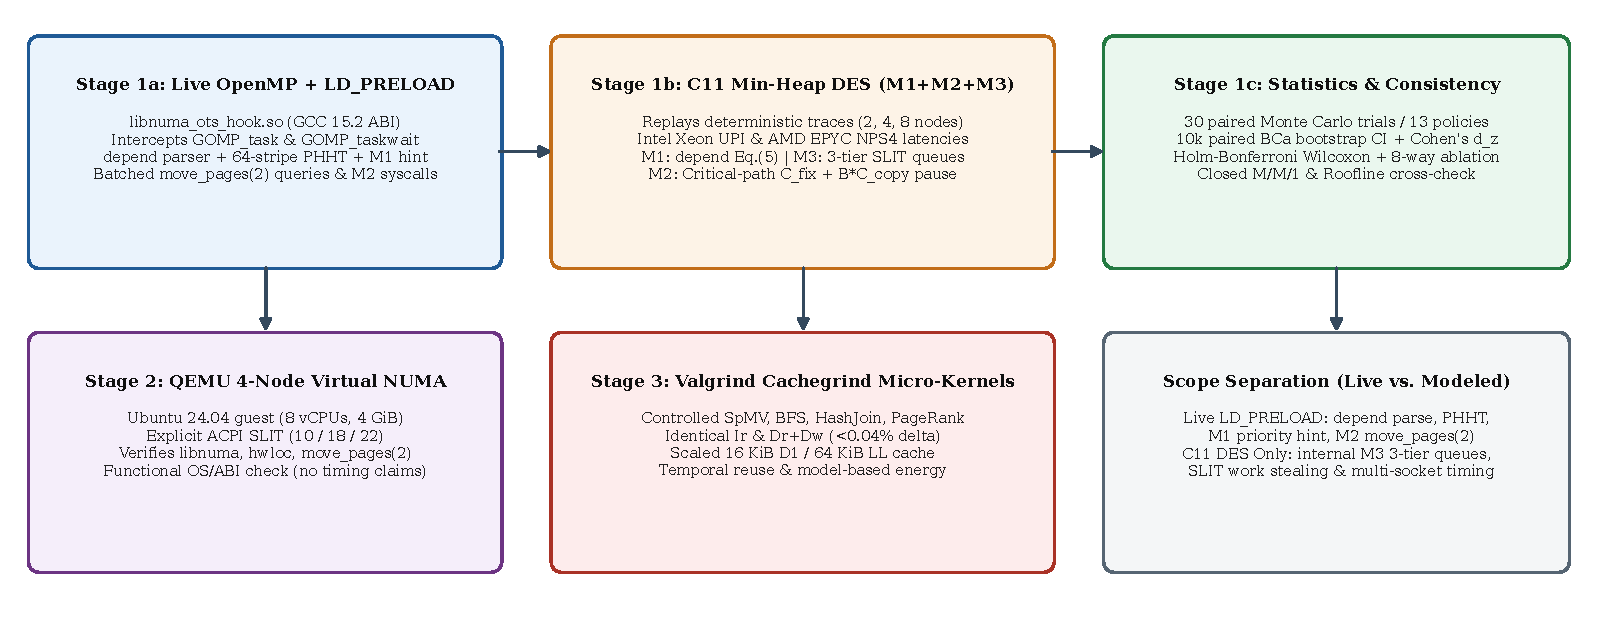
\includegraphics[width=\textwidth]{fig1_architecture.pdf}
\caption{NUMA-OTS architecture and three-stage evaluation methodology. The diagram explicitly separates what executes live inside \texttt{libnuma\_ots\_hook.so} (\texttt{GOMP\_task}/\texttt{GOMP\_taskwait} interception, \texttt{depend} parsing, PHHT lookup, M1 priority hints, and batched \texttt{move\_pages(2)} syscalls) from what is modeled inside the C11 min-heap DES (internal M3 three-tier SLIT queues, closed-form M/M/1 controller queueing, and undiscounted critical-path migration barrier pauses).}
\label{fig:arch}
\end{figure*}

\begin{table}[!t]
\centering
\caption{Summary of Mathematical Notation}
\label{tab:symbols}
\resizebox{\columnwidth}{!}{%
\begin{tabular}{@{}ll|ll@{}}
\toprule
\textbf{Sym.} & \textbf{Definition (Unit)} & \textbf{Sym.} & \textbf{Definition (Unit)} \\
\midrule
$N_{\mathrm{dom}}$ & NUMA domains ($\{2,4,8\}$, impl.\ $\le 8$) & $C_{\mathrm{tot}}$ & Total worker cores ($N_{\mathrm{dom}} \cdot C_{\mathrm{dom}}$) \\
$S_{\mathrm{spd}}$ & Ratio-of-means speedup ($\bar{T}_{\mathrm{base}}/\bar{T}_{\mathrm{OTS}}$) & $\alpha_{\mathrm{loc}}$ & Local DRAM hit fraction \\
$\omega(p)$ & Depend weight (write=2, read=1) & $\eta_{\mathrm{MLP}}$ & Effective MLP overlap factor ($0.55$) \\
$B_{\mathrm{page}}$ & Base page size ($4\text{ KiB}$) & $B_{\mathrm{batch}}$ & Epoch migration batch size ($\le 64$) \\
$\widehat{G}_{p,u\to v}$ & Projected net latency gain (ns) & $\widehat{C}(B)$ & Batch-calibrated migration cost (ns) \\
$\gamma$ & Hysteresis factor ($1.5$) & $T_{\mathrm{cool}}$ & Migration cooldown ($3$ epochs) \\
$L(d,x)$ & Latency, domain $d \to x$ (ns) & $\Delta t$ & Epoch duration (1 taskwait phase) \\
\bottomrule
\end{tabular}%
}
\end{table}

\subsection{First-Touch-Aware Initial Task Placement}
Module M1 moves \emph{tasks} toward the pages placed by OS first touch. For GCC 13.2--15.2 \texttt{GOMP\_task} \cite{ref9}, a read-only parser extracts locator addresses $\{a_1,\dots,a_m\}$ from both legacy ($\texttt{depend[0]} \ne 0$) and extended OpenMP 5.x ($\texttt{depend[0]} = 0$) layouts, skipping \texttt{omp\_all\_memory} tokens. Each locator $a$ is aligned to its 4\,KiB base page:
\begin{equation}
\mathrm{pagebase}(a) = B_{\mathrm{page}} \left\lfloor a / B_{\mathrm{page}} \right\rfloor,
\label{eq:pagebase}
\end{equation}
yielding deduplicated pages $P(T) = \{p_1,\dots,p_k\}$. Virtual-to-domain mappings are cached in a 64-stripe cache-line-padded PHHT with epoch TTL invalidation and in-place updates upon M2 migration, populated on misses via \texttt{move\_pages(..., nodes=NULL)} \cite{ref21}.

For resolved pages $P_{\mathrm{valid}}(T) \subseteq P(T)$, the affinity score of domain $s$ is
\begin{equation}
A(T,s) = \sum_{p \in P_{\mathrm{valid}}(T)} \omega(p)\cdot \mathbb{I}\bigl(\mathrm{PHHT}(p) = s\bigr),
\label{eq:affinity}
\end{equation}
where $\omega(p) = \max_{a_i \in p} \omega_{\mathrm{dep}}(a_i)$ assigns weight $2$ to write/update clauses (\texttt{out}, \texttt{inout}, \texttt{mutexinoutset}, \texttt{inoutset}) and $1$ to read-only (\texttt{in}). Unannotated tasks ($P_{\mathrm{valid}}(T) = \emptyset$) default to Tier~3. Otherwise, with $S^*(T) = \arg\max_s A(T,s)$, the target domain is selected in $O(k)$ time:
\begin{equation}
s^* = \begin{cases}
s_{\mathrm{creator}}, & \text{if } s_{\mathrm{creator}} \in S^*(T), \\
\arg\min_{s \in S^*(T)} q_{\mathrm{len}}(s), & \text{otherwise,}
\end{cases}
\label{eq:target}
\end{equation}
where $q_{\mathrm{len}}(s)$ is domain $s$'s approximate queue depth (maintained via relaxed per-domain atomics cached locally to avoid frequent cross-socket invalidations during ties).

\subsection{Access-Frequency-Based Page Migration}
Let $L(d,x)$ denote the calibrated DRAM latency when a core on domain $d$ misses to memory on domain $x$, and let $\widehat{R}_t(p,d)$ be the projected DRAM miss demand from domain $d$ to page $p$ over one epoch $\Delta t$. Module M2 evaluates the net latency gain of moving $p$ from home $u$ to candidate $v \ne u$:
\begin{equation}
\widehat{G}_{p,u\to v} = \sum_{d=0}^{N_{\mathrm{dom}}-1} \widehat{R}_t(p,d)\,\bigl[L(d,u) - L(d,v)\bigr].
\label{eq:benefit}
\end{equation}
On symmetric topologies (e.g., 2- and 4-socket uniform hops), $\widehat{G}_{p,u\to v} \le 0$ for equally shared pages, suppressing ping-ponging; on asymmetric 8-domain topologies (1-hop vs.\ 2-hop), Eq.~(\ref{eq:benefit}) can still identify a centrally positioned lower-hop domain, which is why the hysteresis and cooldown gates remain essential.

In a hardware Intel Xeon deployment, demand is sampled via \texttt{perf\_event\_open} \cite{ref24} PEBS load-latency events (\texttt{MEM\_TRANS\_RETIRED.LOAD\_LATENCY} \cite{ref25}):
\begin{equation}
R_t^{\mathrm{obs}}(p,d) = \sum_{h \in \mathcal{H}} \sum_{e \in E_t(p,h,d)} P_e \cdot \frac{\tau_{\mathrm{enabled},t}(h)}{\tau_{\mathrm{running},t}(h)},
\label{eq:robs}
\end{equation}
and smoothed via a stabilized EMA with a step-change reset ($\epsilon = 8$, ratio $> 3.0$):
\begin{equation}
\widehat{R}_t(p,d) = \beta_{\mathrm{ema}}\,R_t^{\mathrm{obs}}(p,d) + (1 - \beta_{\mathrm{ema}})\,\widehat{R}_{t-1}(p,d).
\label{eq:ema}
\end{equation}

Because \texttt{move\_pages(2)} executes synchronously with a fixed syscall/locking/IPI TLB-shootdown cost $C_{\mathrm{batch\_fixed}}(N_{\mathrm{dom}})$ \cite{ref26} ($25.6$, $48.0$, and $92.8\,\mu$s on 2, 4, and 8 Xeon domains) plus $C_{\mathrm{copy}} = 1.45\,\mu$s/page, the amortized per-page cost depends directly on the actual batch size $B \in [1, 64]$:
\begin{equation}
\widehat{C}(B) = C_{\mathrm{copy}} + C_{\mathrm{batch\_fixed}}(N_{\mathrm{dom}})/B.
\label{eq:cost}
\end{equation}
At a full batch $B=64$, $\widehat{C}(64) = 1.85$, $2.20$, and $2.90\,\mu$s/page (2N/4N/8N), whereas at a small batch $B=8$ on 8 domains, $\widehat{C}(8)$ rises to $13.05\,\mu$s/page. In our DES, M2 caps each epoch at $B_{\mathrm{epoch}} \le 64$ highest-gain pages and charges the \textbf{full synchronous migration pause} $T_{\mathrm{mig,epoch}} = C_{\mathrm{batch\_fixed}}(N_{\mathrm{dom}}) + B_{\mathrm{epoch}} C_{\mathrm{copy}}$ directly to the phase barrier clock. A page migrates to $v^* = \arg\max_{v \ne u} \widehat{G}_{p,u\to v}$ only if
\begin{equation}
\widehat{G}_{p,u\to v^*} > \gamma\,\widehat{C}(B_{\mathrm{epoch}}),
\label{eq:gate}
\end{equation}
its cooldown $T_{\mathrm{cool}} = 3$ epochs has expired, and destination controller utilization satisfies $\rho_{v^*} < 0.80$.

\noindent\textbf{Proposition 1 (Complexity and Batch-Dependent Break-Even):} \textit{Eqs.~(\ref{eq:affinity})--(\ref{eq:target}) resolve $s^*$ in $O(k)$ time. In the single-consumer regime ($\widehat{R}_t(p,u)=0$) with $\Delta L = L(v^*,u) - L(v^*,v^*) > 0$, Eq.~(\ref{eq:gate}) holds for integer demand counts iff}
\begin{equation}
R_{\min}(B) = \left\lfloor \gamma\,\widehat{C}(B) / \Delta L \right\rfloor + 1.
\label{eq:rmin}
\end{equation}
At $\gamma=1.5$ and $B=64$, $R_{\min}(64) = 43$ (2N), $51$ (4N), $67$ (8N, 1-hop), and $43$ (8N, 2-hop); at $B=8$ on 8N (1-hop), $R_{\min}(8)$ rises sharply to $302$ misses/epoch (plotted across $B \in [4, 64]$ in Fig.~\ref{fig:sens}(b)), showing why batching is vital to amortize TLB shootdowns.

\subsection{Hierarchical Task Queues (Node-Local, Socket-Local, Global)}
To prevent cross-team leakage under nested parallelism, Module M3 maintains per-team queues in three tiers:
\begin{itemize}\setlength{\itemsep}{1pt}\setlength{\parskip}{0pt}\setlength{\topsep}{2pt}
\item \textbf{Tier 1 (node-local per-core deques):} Chase--Lev work-stealing deques \cite{ref27} (LIFO owner pop, FIFO steal) for tasks with $s^* = s_{\mathrm{creator}}$.
\item \textbf{Tier 2 (socket-local per-domain rings):} bounded sequence-stamped MPMC rings (Vyukov's bounded MPMC algorithm \cite{ref28}) for cross-domain tasks ($s^* \ne s_{\mathrm{creator}}$).
\item \textbf{Tier 3 (global team-scoped overflow queue):} unannotated tasks ($P_{\mathrm{valid}}(T) = \emptyset$) and Tier-2 spill-over.
\end{itemize}
Idle workers search in locality-first order: (1)~own Tier-1 deque; (2)~local Tier-2 ring; (3)~intra-domain peer deques; (4)~Tier-3; and (5)~remote Tier-2/Tier-1 queues ordered by ascending $L(d,x)$.

\subsection{Integration with OpenMP Runtime (GNU \texttt{libgomp})}
\textit{Runtime integration scope.} Intercepting public ABI symbols via \texttt{LD\_PRELOAD} (\texttt{GOMP\_task}, \texttt{GOMP\_taskwait}) does not expose \texttt{libgomp}'s internal worker-stealing loop or private queue structures. Therefore:
\begin{itemize}\setlength{\itemsep}{1pt}\setlength{\parskip}{0pt}\setlength{\topsep}{2pt}
\item \textbf{Live \texttt{LD\_PRELOAD} prototype (\texttt{libnuma\_ots\_hook.so}):} intercepts \texttt{GOMP\_task} and \texttt{GOMP\_taskwait}, parses GCC 13.2--15.2 \texttt{depend} locators (\texttt{GOMP\_TASK\_FLAG\_DEPEND = 1<<3}), manages the 64-stripe PHHT via \texttt{SYS\_move\_pages} queries, computes M1 Eq.~(\ref{eq:target}) affinity hints/priority steering, and submits M2 batched \texttt{MPOL\_MF\_MOVE} requests at \texttt{GOMP\_taskwait} while verifying per-page kernel \texttt{status} codes.
\item \textbf{Internal \texttt{libgomp} requirement (modeled in DES):} full M3 three-tier queues, domain-pinned task insertion, SLIT-ordered work stealing, and OpenMP 5.2 TSC-deferred subqueues (Sec.~12.9 \cite{ref8}) require modifying \texttt{libgomp.so.1} (or LLVM \texttt{libomp}) internally; in this study, M1+M2+M3 scheduling and multi-socket performance are evaluated inside the C11 DES.
\end{itemize}

% ===========================================================================
\section{Implementation Details}

\subsection{Runtime Modifications and Hooks}
Our evaluation spans three decoupled stages (exact source filenames and reproducibility scripts are packaged in the companion artifact):
\begin{enumerate}\setlength{\itemsep}{1pt}\setlength{\parskip}{0pt}\setlength{\topsep}{2pt}
\item \textbf{Stage~1 --- Live \texttt{LD\_PRELOAD} prototype, OpenMP trace extraction, and C11 DES.} Stage~1a runs four live OpenMP task benchmarks under \texttt{LD\_PRELOAD=./libnuma\_ots\_hook.so} on the host system, verifying ABI parsing, PHHT caching, and \texttt{move\_pages(2)} syscall submission while generating deterministic synthetic logical-page footprint traces \texttt{(array\_id << 16) | (offset >> 12)}. Stage~1b replays these traces in a pure-C11 min-heap DES across 2, 4, and 8 NUMA domains ($C_{\mathrm{dom}}=4$ cores/domain, $C_{\mathrm{tot}} \in \{8, 16, 32\}$ cores). Each phase executes $10$ inner sweeps so that iterative phases span multi-millisecond intervals ($\Delta t \approx 1$--$4$\,ms) and full synchronous \texttt{move\_pages(2)} barrier pauses ($C_{\mathrm{batch\_fixed}} + B_{\mathrm{epoch}} C_{\mathrm{copy}}$) are charged directly to the barrier clock. Stage~1c computes 10,000-resample paired BCa bootstrap CIs, Holm--Bonferroni Wilcoxon tests, Cohen's $d_z$, 13-policy ablations, and vector PDF figures.
\item \textbf{Stage~2 --- Optional 4-node QEMU virtual NUMA verification.} The companion artifact includes host/guest scripts for booting an Ubuntu 24.04 Linux guest with 4 virtual NUMA nodes (8 vCPUs, 4\,GiB RAM, ACPI SLIT distances 10/18/22) to functionally test \texttt{numactl --hardware}, \texttt{lstopo}, batched \texttt{move\_pages(2)} PHHT queries, and kernel physical page relocation (\texttt{MPOL\_MF\_MOVE}); QEMU is intended strictly for functional OS/syscall checks rather than timing and was not pre-executed on the WSL2 host.
\item \textbf{Stage~3 --- Single-hierarchy cache-reuse micro-benchmarks under Valgrind Cachegrind.} We run controlled OpenMP micro-kernels (identical arrays and checksums, with instruction counts differing by at most $0.033\%$, i.e., $<0.04\%$, across \texttt{base} and \texttt{ots}) under Valgrind Cachegrind (\texttt{--cache-sim=yes}, scaled 16\,KiB D1 and 64\,KiB unified LL cache) to isolate the effect of fixed-partition temporal cache reuse (\texttt{ots}) versus cyclic partition rotation (\texttt{base}), paired with a model-based energy estimate ($E = 0.42\,I_r + 1.8\,D_{1m} + 35\,\mathrm{LL}_m$\,nJ). This stage isolates single-hierarchy reuse rather than running the full multi-socket M1+M2+M3 scheduler.
\end{enumerate}

\subsection{Data Structures and Overhead Analysis}
\textit{Data structures and bounds.} The PHHT uses 16,384 open-addressed slots (64 lock stripes in the live hook) with Knuth multiplicative hashing and $\le 64$ probes; each 160-byte entry stores page key, home/cached node, timestamps, and 8-element demand vectors (2.6\,MB total; current implementation supports $N_{\mathrm{dom}} \le 8$). Tier-1/2/3 queues are 2,048-entry circular buffers, and the DES core-completion queue is a binary min-heap of size $C_{\mathrm{tot}} \le 32$ (phase barriers and M2 epochs execute sequentially between min-heap drains at each phase boundary).

\textit{Overhead accounting and live hook telemetry.} Modeled scheduling and synchronous migration overhead for Full NUMA-OTS is \OvhdRangeAll{} across all 12 configurations (\OvhdRangeEight{} on 8 domains). On the WSL2 host (\hostgcc{}, $1$ physical \texttt{sysfs} NUMA node configured with $4$ logical domains, \texttt{pmu\_supported=0}), \texttt{libnuma\_ots\_hook.so} \HookSummaryText{}. This host run verifies ABI interception, PHHT metadata lookups, and \texttt{move\_pages(2)} request submission rather than physical cross-node relocation. Note that $99.93\%$ of extracted tasks carry \texttt{depend} locators, so Tier-3 overflow is only lightly exercised in these traces, and because each task carries at most two \texttt{depend} locators, per-task \texttt{GOMP\_task} miss queries remain small ($\approx 1.1$ pages/syscall, amortized by the $>82\%$ PHHT hit ratio), whereas epoch migrations batch multiple hot pages at \texttt{GOMP\_taskwait} (\BatchHistSummary{}).

\begin{table}[!t]
\centering
\caption{Simulator Parameters (Identical Across Policies Unless Noted)}
\label{tab:params}
\resizebox{\columnwidth}{!}{%
\begin{tabular}{@{}ll@{}}
\toprule
\textbf{Parameter} & \textbf{Value} \\
\midrule
Topologies & 2, 4, 8 domains $\times$ 4 cores ($C_{\mathrm{tot}} \in \{8, 16, 32\}$); Xeon UPI \& EPYC NPS4 \\
Latency $L(d,x)$ (Xeon / EPYC) & Local 84 / 88 ns; 1-hop 149 / 138 ns; 2-hop 186 / 208 ns \\
Compute rate / MLP $\eta_{\mathrm{MLP}}$ & 0.45 ns per \texttt{work\_op} / $0.55$; 10 inner sweeps per phase ($\Delta t \approx 1$--$4$\,ms) \\
Misses/page (nominal; swept $[2,100]$) & SpMV 18, BFS 28, HashJoin 22, PageRank 20 ($\times 10$ sweeps/phase) \\
Closed M/M/1 controller model & $T_{\mathrm{cont}}(s) = 12\rho_s/(1-\rho_s)$ ns, $\rho_s = \min(M_s/C_{\mathrm{bw}}, 0.88)$, $C_{\mathrm{bw}} = 180{,}000$ misses/phase \\
Dispatch cost & OTS 145 ns (+6 ns/PMU sample); ParFT $105+14N_{\mathrm{dom}}$ ns; central $110+18N_{\mathrm{dom}}$ ns \\
Critical-path M2 barrier pause & Exact undiscounted $C_{\mathrm{batch\_fixed}}(N_{\mathrm{dom}}) + B_{\mathrm{epoch}} \cdot 1.45\,\mu$s ($B_{\mathrm{epoch}} \le 64$) \\
M2 (Full / Ungated) & $\gamma$ = 1.5 / 1.0; $T_{\mathrm{cool}}$ = 3 / 0 epochs; util.\ guard $\rho < 0.80$ / $0.99$ \\
M2 predictor & $P_{\mathrm{pmu}}=16$; $\beta_{\mathrm{ema}}=0.3$; reset ratio 3.0; $\epsilon = 8$ \\
Mixed first-touch (swept $0\%$--$100\%$) & 80\% of shared $x$, \texttt{dist}, hash-table, \texttt{pr\_cur} pages on Node 0; partition pages distributed \\
Seeds & splitmix64 + xorshift64*; shared across all 13 policies per trial \\
\bottomrule
\end{tabular}%
}
\end{table}

\subsection{Compatibility with Existing OpenMP Constructs}
Our automated 8-test verification suite (compiled and passed both natively and under \texttt{-fsanitize=address,undefined} on \hostgcc{}) validates: (T1)~8-thread 64-stripe PHHT concurrency and TTL expiry; (T2)~GCC 13.2--15.2 legacy and OpenMP 5.x \texttt{depend} ABI layouts and \texttt{omp\_all\_memory}; (T3)~M1 Eq.~(\ref{eq:target}) tie-breaking; (T4)~M2 Proposition~1 $R_{\min}(B)$ batch-size calibration ($B \in \{8, 64\}$) and EMA step-change guard; (T5)~OpenMP 5.2 \texttt{depend(in/out/inout/mutexinoutset/inoutset)}, \texttt{taskgroup}, \texttt{taskloop reduction}, \texttt{if(0)} undeferred execution, and \texttt{final(1)}; (T6)~\texttt{untied} tasks and detachable tasks (\texttt{detach} + \texttt{omp\_fulfill\_event}); (T7)~nested \texttt{omp parallel} teams and \texttt{cancel taskgroup}; and (T8)~asymmetric task-tree liveness without deadlock or starvation.

% ===========================================================================
\section{Experimental Evaluation}

\subsection{Hardware Platforms (4-Socket, 8-Socket, AMD EPYC, Intel Xeon)}
\textit{Simulated multi-socket targets.} We evaluate two calibrated architectures across 2, 4, and 8 NUMA domains ($C_{\mathrm{tot}} \in \{8, 16, 32\}$ cores): (i)~\textbf{Intel Xeon (Cooper Lake UPI)} ($T_{\mathrm{loc}} = 84$\,ns, 1-hop $149$\,ns, 2-hop $186$\,ns; 8-domain mean remote $\overline{T}_{\mathrm{rem}} = 170.1$\,ns, ratio $\overline{T}_{\mathrm{rem}}/T_{\mathrm{loc}} = 2.025$) and (ii)~\textbf{AMD EPYC (Milan/Rome NPS4 Infinity Fabric)} ($T_{\mathrm{loc}} = 88$\,ns, intra-socket 1-hop $138$\,ns, cross-socket 2-hop $208$\,ns; 8-domain mean remote $\overline{T}_{\mathrm{rem}} = (3\cdot 138 + 4\cdot 208)/7 = 178.0$\,ns, ratio $\overline{T}_{\mathrm{rem}}/T_{\mathrm{loc}} = 2.023$). \textit{Experimental host.} Stage~1 trace extraction and Stage~3 Cachegrind ran on \hostcpu{} under \hostos{} with \hostgcc{} ($1$ physical NUMA node, no hardware PEBS); raw 30-trial logs for both Intel Xeon and AMD EPYC are archived in the companion artifact.

\subsection{Benchmark Suite: SpMV, BFS, Hash Join, PageRank}
We evaluate four OpenMP task workloads using deterministic synthetic logical-page footprint traces ($1{,}542$--$1{,}932$ unique 4\,KiB logical pages per workload, i.e., $6.0$--$7.6$\,MiB logical footprint) modeling the task-level locality and phase-reuse patterns of larger server-scale datasets exceeding per-socket LLC capacity:
(a)~\textbf{CSR SpMV} \cite{ref29}: 32,768 rows, 8 non-zeros/row, 256-row tasks across 8 phases ($1{,}024$ tasks = $128$ tasks/phase = $4.0$ tasks/worker/phase on 32 cores);
(b)~\textbf{Level-synchronous frontier BFS} \cite{ref30}: 32,768 vertices (degree 12), 512 roots, 256-vertex frontier chunks across up to 8 levels ($129$ total tasks $\approx 16.1$ tasks/level = \textbf{$0.50$ tasks/worker/level} on 32 cores, exhibiting limited parallelism);
(c)~\textbf{Morsel-driven hash join} \cite{ref31}: 131,072 probe tuples against a 32,768-tuple build table across 6 phases ($768$ tasks = $128$ tasks/phase = $4.0$ tasks/worker/phase); and
(d)~\textbf{Iterative PageRank}: 32,768 vertices, in-degree 8, 256-vertex tasks across 8 damping iterations ($1{,}024$ tasks = $128$ tasks/phase = $4.0$ tasks/worker/phase).

\subsection{Metrics: Runtime, Remote Access Ratio, Cache Miss Rate, Energy}
In Stage~1 (C11 DES), we report: (i)~simulated runtime (mean $\pm \sigma$) and ratio-of-means speedup $S_{\mathrm{spd}} = \bar{T}_{\mathrm{base}}/\bar{T}_{\mathrm{OTS}}$; (ii)~remote DRAM access ratio $1 - \alpha_{\mathrm{loc}}$; (iii)~closed-form controller queueing delay $T_{\mathrm{cont}}$ (Table~\ref{tab:ctrl}); (iv)~\textbf{extended 6-epoch re-migrations} (twice the $T_{\mathrm{cool}}=3$ window) and \textbf{beneficial migration precision} (\% of migrated pages whose remote misses decrease in the next phase); (v)~synchronous migration pause (ms) and total overhead (\%); and (vi)~Stage~1 DES per-domain LLC miss rate and model-based \textbf{dynamic} vs.\ \textbf{total} (static leakage $18$\,W/domain $\times T_{\mathrm{makespan}}$ + dynamic) energy estimates. Separately, in Stage~3 (single-hierarchy Valgrind Cachegrind with scaled 16\,KiB D1 and 64\,KiB unified LL caches), instruction and data-reference counts match within $0.04\%$ (max $0.033\%$ on BFS), isolating fixed-partition temporal-reuse LL reductions and model-based energy estimates ($E = 0.42\,I_r + 1.8\,D_{1m} + 35\,\mathrm{LL}_m$\,nJ; \cgSpmvLthree{}; \cgBfsLthree{}; \cgJoinPrLthree{}; \cgEnergySummary{}). Stage~3 values are model-based single-cache estimates distinct from Stage~1 DES LLC rates and physical hardware power measurements.

\begin{table}[!t]
\centering
\caption{Closed-Form 8-Domain DRAM Controller Accounting (\texttt{Base} $\to$ \texttt{Full OTS}): Exact Unique Pages, Node-0 Pages, Effective Misses/Page, Phase-Mean Node-0 Misses $M_0$ ($C_{\mathrm{bw}}=180\text{k}$), Phase-Mean Utilization $\rho_0 = \min(M_0/C_{\mathrm{bw}}, 0.88)$, and Phase-Mean $T_{\mathrm{cont}}(0) = E[12\rho_0/(1-\rho_0)]$ (ns; convex across uneven BFS frontiers and M2 convergence phases)}
\label{tab:ctrl}
\resizebox{\columnwidth}{!}{%
\begin{tabular}{@{}lccccccc@{}}
\toprule
\textbf{Workload} & \textbf{Tasks} & \textbf{Pages} & \textbf{Node-0 Pgs} & \textbf{Miss/Pg} & \textbf{$M_0$ / Phase} & $\boldsymbol{\rho_0}$ & $\boldsymbol{T_{\mathrm{cont}}(0)}$ \\
\midrule
\ControllerAccountingRows
\bottomrule
\end{tabular}%
}
\end{table}

\subsection{Comparison: Default OpenMP, \texttt{numactl}, NUMA-OTS}
Each workload--domain configuration runs $n = 30$ paired trials across 13 policies (Table~\ref{tab:ablation}), including \texttt{numactl}-equivalent \texttt{Mem0}/\texttt{Inter}, static \texttt{ParFT}, reactive \texttt{AutoNUMA}, individual/pairwise ablations (\texttt{M1}, \texttt{M2}, \texttt{M3}, \texttt{M1+M2}, \texttt{M1+M3}, \texttt{M2+M3}), \texttt{Ungated M2}, and \texttt{Full NUMA-OTS}. We compute 95\% paired BCa bootstrap CIs (10,000 resamples, seed 42) for the ratio of paired means $\bar{T}_{\mathrm{base}}/\bar{T}_{\mathrm{OTS}}$, paired Cohen's $d_z$, and exact one-sided paired Wilcoxon signed-rank $p$-values (testing $T_{\mathrm{base}} > T_{\mathrm{OTS}}$) with Holm--Bonferroni correction across the 12-configuration family (tied exact ranks yield identical minimum $p$-values across several configurations).

\begin{table*}[!t]
\centering
\caption{Simulated Mean Execution Time (ms $\pm \sigma$) over 30 Paired Trials on 2, 4, and 8 NUMA Domains; Ratio-of-Means Speedup with 95\% Paired BCa Bootstrap CIs, Paired Cohen's $d_z$, Holm--Bonferroni Wilcoxon $p$-Values (12-Test Family), and Internal Roofline Prediction (with Exact \% Discrepancy)}
\label{tab:speedup}
\resizebox{\textwidth}{!}{%
\begin{tabular}{@{}lccccccccccc@{}}
\toprule
\textbf{Workload (N)} & \textbf{Base ($\pm\sigma$)} & \textbf{ParFT} & \textbf{Inter} & \textbf{AutoN} & \textbf{M1+M3} & \textbf{Ungat} & \textbf{Full OTS ($\pm\sigma$)} & \textbf{Speedup [95\% CI]} & $\boldsymbol{d_z}$ & $\boldsymbol{p_{\mathrm{Holm}}}$ & \textbf{Roofline (Err)} \\
\midrule
\MainSpeedupRows
\bottomrule
\end{tabular}%
}
\end{table*}

\begin{table}[!t]
\centering
\caption{Complete 8-Domain Component Ablation (Speedup vs.\ \texttt{Base} and $\alpha_{\mathrm{loc}}$ Across All 13 Policies, 30 Trials)}
\label{tab:ablation}
\resizebox{\columnwidth}{!}{%
\begin{tabular}{@{}lcccc@{}}
\toprule
\textbf{Policy (8 Domains)} & \textbf{SpMV} & \textbf{BFS} & \textbf{HashJoin} & \textbf{PageRank} \\
\midrule
\AblationRows
\bottomrule
\end{tabular}%
}
\end{table}

\begin{figure*}[!t]
\centering
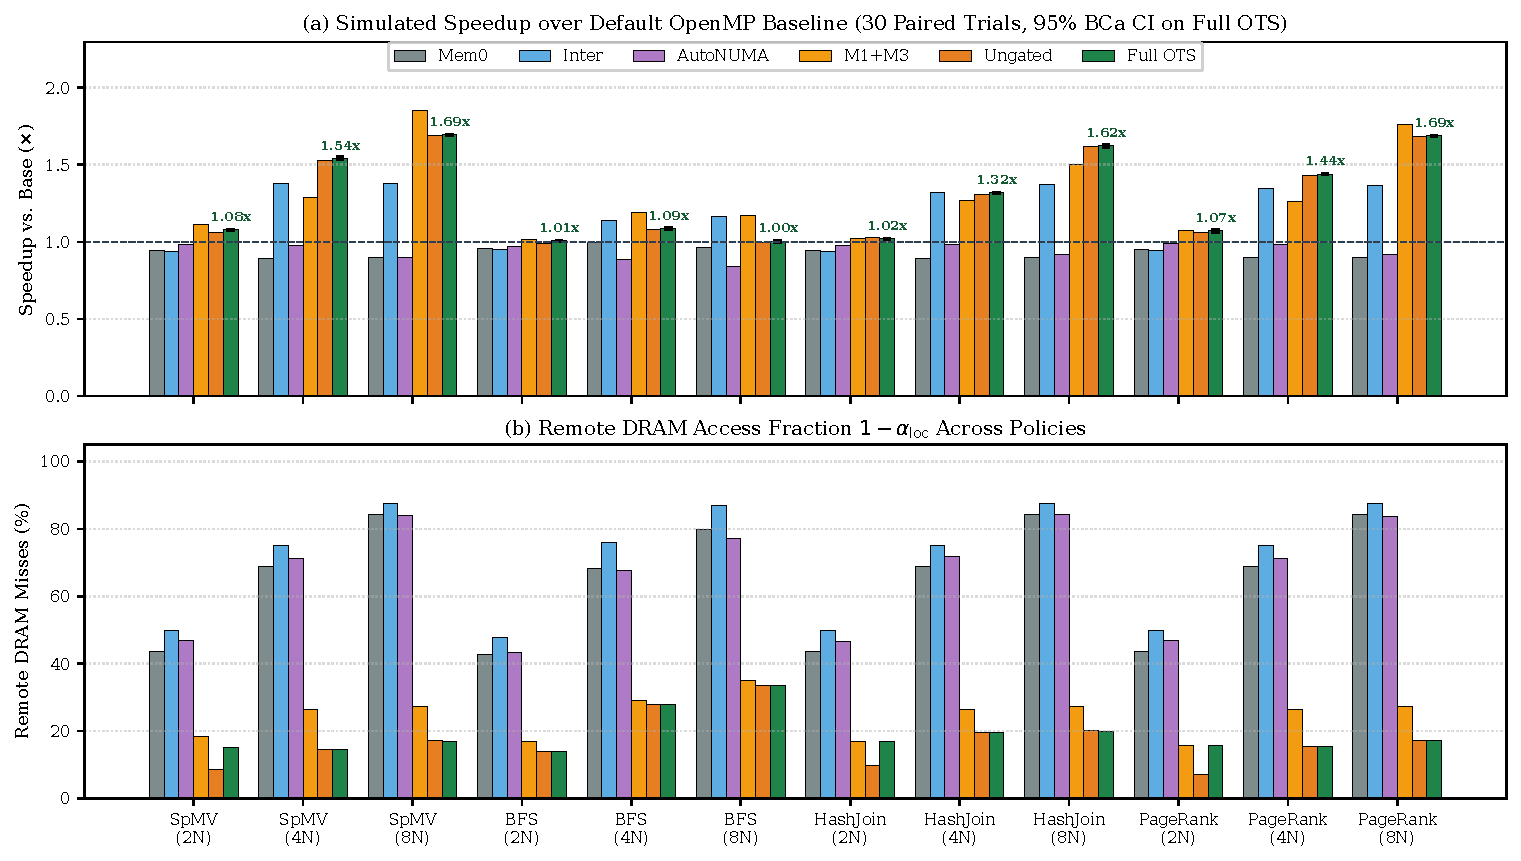
\includegraphics[width=\textwidth]{fig2_evaluation.pdf}
\caption{Simulation results on 2, 4, and 8 NUMA domains (30 paired trials per bar): (a)~speedup of \texttt{Mem0}, \texttt{Inter}, \texttt{AutoNUMA}, \texttt{M1+M3}, \texttt{Ungated}, and \texttt{Full OTS} over the default OpenMP baseline, with 95\% paired BCa CIs on Full OTS; (b)~remote DRAM access fraction $1 - \alpha_{\mathrm{loc}}$.}
\label{fig:eval}
\vspace{0.35em}
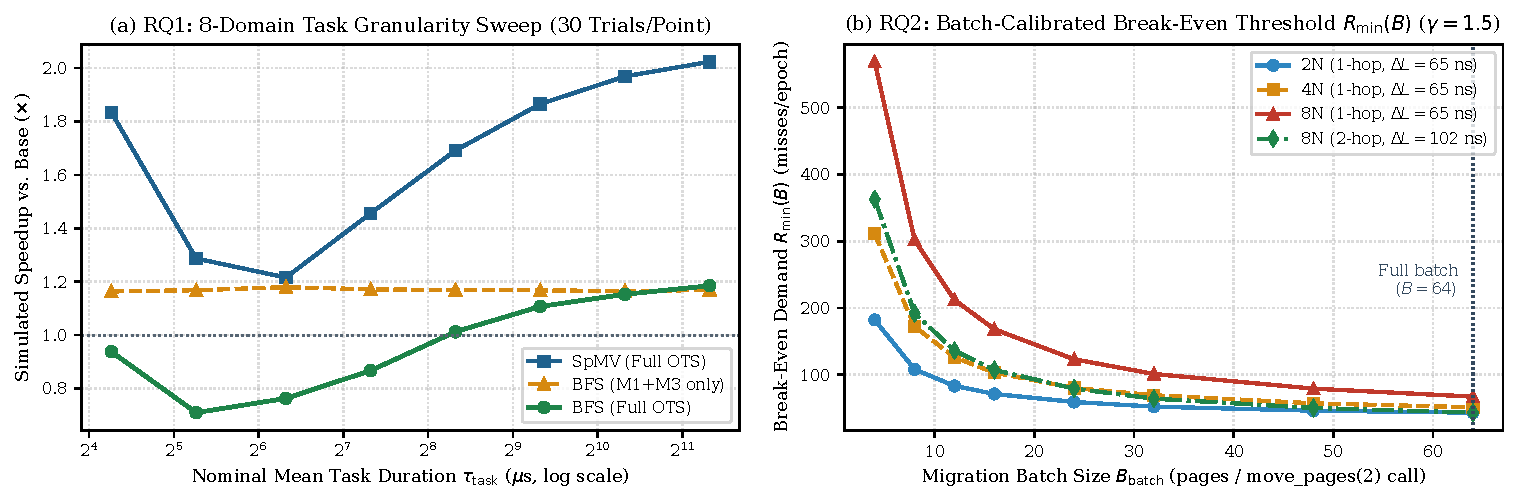
\includegraphics[width=\textwidth]{fig3_sensitivity.pdf}
\caption{Sensitivity analysis: (a)~RQ1 30-trial task-granularity sweep on 8-domain BFS and SpMV; (b)~RQ2 batch-size-calibrated break-even demand $R_{\min}(B)$ from Eq.~(\ref{eq:rmin}) at $\gamma=1.5$ across actual migration batch sizes $B_{\mathrm{batch}} \in [4, 64]$, demonstrating how small batches inflate $R_{\min}$.}
\label{fig:sens}
\end{figure*}

\textit{End-to-end speedups and component ablation.} Tables~\ref{tab:speedup}--\ref{tab:ablation} and Fig.~\ref{fig:eval} reveal four findings:
\begin{itemize}\setlength{\itemsep}{1pt}\setlength{\parskip}{0pt}\setlength{\topsep}{2pt}
\item \textbf{Iterative workloads (SpMV, PageRank, HashJoin):} Full NUMA-OTS scales monotonically with domain count, achieving \SpmvSpdAll{} on SpMV, \PrSpdAll{} on PageRank, and \JoinSpdAll{} on HashJoin ($p_{\mathrm{Holm}} = 1.12 \times 10^{-8}$), consistently outperforming \texttt{Mem0} (\MemZeroBeatRange{}) and reactive \texttt{AutoNUMA} (\AutoNumaBeatRange{}, which lacks M1 \texttt{depend} routing and incurs fault-driven migration overhead). Across 4- and 8-domain iterative workloads, Full NUMA-OTS outperforms \texttt{Interleave} by $1.11\times$--$1.24\times$ and static \texttt{ParFT} by $1.17\times$--$1.39\times$ (whereas on 8-domain BFS, unamortized M2 pauses reduce Full NUMA-OTS relative to \texttt{Interleave} to $0.86\times$, while \texttt{M1+M3} matches or beats \texttt{Interleave} on all workloads).
\item \textbf{Component isolation and synchronous migration cost (Table~\ref{tab:ablation}):} On 8 domains, \texttt{M1 only} delivers the largest single-module speedup ($1.14\times$--$1.45\times$) by routing tasks to partition pages; adding \texttt{M3} eliminates cross-socket stealing interference (lifting \texttt{M1+M3} to $1.50\times$--$1.85\times$ on iterative workloads and $1.17\times$ on BFS). Adding gated \texttt{M2} lifts $\alpha_{\mathrm{loc}}$ further to \AlphaOtsEightIterRange{}, yielding a clear net speedup over \texttt{M1+M3} on all 4-domain iterative workloads (SpMV $14.62$ vs.\ $17.54$\,ms; HashJoin $15.51$ vs.\ $16.15$\,ms; PageRank $17.73$ vs.\ $20.21$\,ms) and on controller-bound 8-domain HashJoin ($7.28$ vs.\ $7.85$\,ms, $1.62\times$ vs.\ $1.50\times$). By contrast, on 8-domain SpMV and PageRank, the synchronous 8-domain TLB-shootdown pause ($1.42$\,ms, $16.8\%$--$19.0\%$ of makespan) exceeds the marginal latency gain from raising $\alpha_{\mathrm{loc}}$ from $72.7\%$ to $82.9\%$, leaving placement-only \texttt{M1+M3} ($1.85\times$ and $1.76\times$) faster than synchronous \texttt{Full OTS} ($1.69\times$ and $1.69\times$).
\item \textbf{BFS negative migration regime \& Roofline failure:} On BFS, Full NUMA-OTS achieves \BfsSpdAll{} (8N non-significant, $p_{\mathrm{Holm}}=0.159$), whereas placement-only \texttt{M1+M3} achieves \BfsMthirteenAll{}. The internal Roofline check predicts \BfsRfPredEight{} on 8-domain BFS---a \textbf{\BfsRfErrEight{} discrepancy} (compared to \IterRfErrRange{} across SpMV, HashJoin, and PageRank, where 8N discrepancies also reflect unmodeled synchronous migration pauses in Eq.~\ref{eq:roofline}). Two physical mechanisms explain the BFS discrepancy: (i)~BFS averages only \textbf{$0.50$ tasks/worker/level} on 32 cores (causing severe barrier idle time omitted by Eq.~\ref{eq:roofline}), and (ii)~synchronous \texttt{move\_pages(2)} barrier pauses ($0.599$\,ms, $16.9\%$ of makespan) cannot amortize over sparse frontier levels.
\item \textbf{Intel Xeon vs.\ AMD EPYC:} On 8-domain AMD EPYC, Full NUMA-OTS achieves \EpycEightSummary{}, closely tracking Intel Xeon precisely because their 8-domain mean remote/local ratios are nearly identical ($2.023$ vs.\ $2.025$), while EPYC's wider intra- vs.\ inter-socket asymmetry ($138$ vs.\ $208$\,ns) increases the benefit of SLIT-ordered M3 stealing.
\end{itemize}

\begin{table}[!t]
\centering
\caption{8-Domain Simulated Telemetry: Locality, Queueing, Extended 6-Epoch Re-Migrations, Migration Precision, Barrier Pause, Stage~1 DES LLC Miss Rate, and Model-Based Dynamic vs.\ Total Energy}
\label{tab:telemetry}
\resizebox{\columnwidth}{!}{%
\begin{tabular}{@{}lcccc@{}}
\toprule
\textbf{Metric (8-Domain Topology)} & \textbf{SpMV} & \textbf{BFS} & \textbf{HashJoin} & \textbf{PageRank} \\
\midrule
\TelemetryEightNodeRows
\bottomrule
\end{tabular}%
}
\end{table}

\textit{Telemetry and energy estimates.} Table~\ref{tab:telemetry} shows that on 8 domains, Full NUMA-OTS cuts $T_{\mathrm{cont}}$ from \TcontBaseEightRange{} to \TcontOtsEightRange{} (\TcontRedRange{} reduction, auditable via Table~\ref{tab:ctrl}), reduces Stage~1 DES LLC miss rates from \DesLlcBaseRange{} to \DesLlcOtsRange{}, reduces model-based \textbf{dynamic} memory/interconnect energy by \DynEnergyRedRange{} (independently of runtime scaling), and reduces \textbf{total} estimated energy (static leakage + dynamic) by \TotEnergyRedRange{} across all four workloads (\TotEnergyRedIterRange{} on SpMV/HashJoin/PageRank and \TotEnergyRedBfs{} on BFS, where static race-to-halt savings track makespan reduction).

\subsection{Sensitivity: Task Granularity, Migration Threshold}
\textit{RQ1 (granularity).} Fig.~\ref{fig:sens}(a) plots the 30-trial granularity sweep on 8-domain BFS and SpMV: \GranSweepSummary{}. The non-monotonic dip at intermediate task durations ($\tau_{\mathrm{task}} \approx 38$--$80\,\mu\mathrm{s}$) occurs because page demand begins crossing the $R_{\min}(B)$ migration threshold and triggering synchronous barrier pauses before phases are long enough to amortize the fixed TLB-shootdown cost, whereas at $\tau_{\mathrm{task}} = 19\,\mu\mathrm{s}$ fewer pages qualify for migration and above $320\,\mu\mathrm{s}$ phase duration amortizes the pause. Placement-only \texttt{M1+M3} stays positive across all granularities, whereas synchronous M2 requires sufficiently long tasks and phases to amortize its barrier pause.

\textit{RQ2 (migration stability \& parameter sweeps).} Because a 2-epoch window is blocked by $T_{\mathrm{cool}}=3$, Table~\ref{tab:telemetry} evaluates \textbf{extended 6-epoch re-migrations} (twice the cooldown) and \textbf{beneficial migration precision}: \ReSixSummary{}. Across our parameter sensitivity sweeps, \SensSweepSummary{}. Fig.~\ref{fig:sens}(b) plots Eq.~(\ref{eq:rmin}) across batch sizes $B \in [4, 64]$.

% ===========================================================================
\section{Discussion}

\subsection{When NUMA-Awareness Matters Most}
Within our simulated multi-socket regimes, NUMA-OTS delivers its largest gains when three conditions coincide: (1)~sufficient parallelism per phase ($\ge 2$--$4$ tasks/worker/phase) so cores are not barrier-starved; (2)~memory-bound execution ($f_{\mathrm{mem}} \ge 0.60$) with multi-domain latency asymmetry ($N_{\mathrm{dom}} \ge 4$); and (3)~reusable hot data whose demand exceeds the batch-calibrated threshold $R_{\min}(B)$. By contrast, under-parallelized frontier graphs (8-domain BFS at $0.50$ tasks/worker/level) and 8-domain workloads whose TLB-shootdown pauses approach $17\%$--$19\%$ of makespan favor placement-only \texttt{M1+M3} over synchronous barrier migration unless migration is executed asynchronously or amortized over longer phases ($\tau_{\mathrm{task}} \ge 1$\,ms).

\subsection{Overhead vs.\ Benefit Trade-offs}
Charging full synchronous \texttt{move\_pages(2)} pauses shows that M2 is net-positive primarily when migration batches approach $B_{\mathrm{batch}} \approx 32$--$64$ pages and phases span multiple milliseconds ($\Delta t \ge 1$\,ms). Comparing Full NUMA-OTS against reactive \texttt{AutoNUMA} (Table~\ref{tab:ablation}) highlights that coordinating task placement (M1+M3) with batched migration (M2) avoids the page-fault overhead and task-page chasing inherent in task-blind OS migration.

\subsection{Portability and Limitations}
First, this is a \textbf{simulation-based study} calibrated to published Intel Xeon and AMD EPYC latencies \cite{ref6,ref18,ref25}, not a bare-metal multi-socket hardware evaluation; narrow bootstrap CIs reflect low Monte Carlo variance within the simulator rather than hardware noise. Second, while \texttt{libnuma\_ots\_hook.so} verifies live GCC 15.2.0 \texttt{depend} parsing, PHHT caching, and \texttt{move\_pages(2)} request submission on WSL2 (1 physical node), physical cross-node migration requires a multi-node Linux kernel (e.g., via the optional Stage~2 QEMU scripts), and full M3 three-tier work stealing requires patching \texttt{libgomp.so.1} or LLVM \texttt{libomp} internally. Third, our Stage~1 DES uses synthetic logical-page traces and calibrated \texttt{misses/page} inputs (mitigated by our $[2, 100]$ misses/page and $[0.20, 0.95]$ $f_{\mathrm{mem}}$ sweeps), Stage~3 Valgrind Cachegrind models a single scaled cache hierarchy rather than multi-socket coherence directories, and energy numbers are model-based estimates rather than direct RAPL/electrical measurements.

% ===========================================================================
\section{Conclusion and Future Work}

\subsection{Summary}
We presented a simulation-based design and evaluation of NUMA-OTS, combining \texttt{depend}-guided task placement (M1), batch-calibrated cost-benefit page migration (M2), and topology-aligned three-tier queues (M3), supported by a live \texttt{LD\_PRELOAD} ABI/syscall prototype. Within our calibrated 2-, 4-, and 8-domain simulations across SpMV, BFS, HashJoin, and PageRank, Full NUMA-OTS achieves speedups of \SpdRangeAll{} (\SpdRangeIterEight{} on 8-domain iterative workloads; significant on 11 of 12 configurations, \MaxPHolmSig{}), outperforms \texttt{Mem0} and reactive \texttt{AutoNUMA} across all configurations, reduces controller queueing by \TcontRedRange{}, and identifies both the regimes where synchronous M2 excels (4-domain iterative workloads and controller-bound 8-domain HashJoin) and the regimes where placement-only \texttt{M1+M3} outperforms synchronous migration (8-domain BFS at $0.50$ tasks/worker/level and 8-domain SpMV/PageRank under high synchronous TLB-shootdown costs).

\subsection{Extensions: NUMA-Aware GPU Offloading, CXL Memory Pooling}
Future work will integrate M3's three-tier queues directly into patched GNU \texttt{libgomp.so.1} and LLVM \texttt{libomp} on bare-metal multi-socket Xeon and EPYC servers with hardware PEBS and RAPL MSRs \cite{ref32}, extend M1 affinity scoring to OpenMP \texttt{target} GPU offloading across NUMA-attached PCIe/NVLink topologies, and generalize M2's batch-calibrated migration gate to tiered CXL memory pooling \cite{ref33}.

\noindent\textbf{Reproducibility:} All C11/Python sources, 8-test ASan/UBSan suite, deterministic traces (SHA-256), raw CSVs, and figure scripts are publicly available at \url{https://github.com/MohaSeyam/NUMA-OTS}; running \texttt{./scripts/run\_all.sh 30} and \texttt{./scripts/run\_stage3\_sniper.sh} regenerates every table and figure.

\noindent\textbf{Acknowledgments:} The authors thank the Computer Engineering Department at the Islamic University of Gaza for academic support.

% ===========================================================================
\renewcommand{\refname}{9.\quad References}
{\footnotesize
\begin{thebibliography}{99}\setlength{\itemsep}{0pt}\setlength{\parskip}{0pt}
\bibitem{ref1} J. L. Hennessy and D. A. Patterson, \textit{Computer Architecture: A Quantitative Approach}, 6th ed. Cambridge, MA, USA: Morgan Kaufmann, 2017.
\bibitem{ref2} A. Grama, A. Gupta, G. Karypis, and V. Kumar, \textit{Introduction to Parallel Computing}, 2nd ed. Boston, MA, USA: Addison-Wesley, 2003.
\bibitem{ref3} C. Lameter, ``NUMA (Non-Uniform Memory Access): An overview,'' \textit{ACM Queue}, vol. 11, no. 7, pp. 40--51, Jul. 2013, doi: 10.1145/2508834.2513149.
\bibitem{ref4} W. A. Wulf and S. A. McKee, ``Hitting the memory wall: Implications of the obvious,'' \textit{ACM SIGARCH Comput. Archit. News}, vol. 23, no. 1, pp. 20--24, Mar. 1995, doi: 10.1145/216585.216588.
\bibitem{ref5} M. Diener, E. H. M. Cruz, L. L. Pilla, F. Dupros, and P. O. A. Navaux, ``Characterizing communication and page usage of parallel applications for thread and data mapping,'' \textit{Perform. Eval.}, vols. 88--89, pp. 18--36, Jun. 2015, doi: 10.1016/j.peva.2015.03.001.
\bibitem{ref6} M. Dashti et al., ``Traffic management: A holistic approach to memory placement on NUMA systems,'' in \textit{Proc. ACM ASPLOS}, Mar. 2013, pp. 381--394, doi: 10.1145/2451116.2451157.
\bibitem{ref7} Linux Kernel Development Community, \textit{NUMA Memory Policy and AutoNUMA Balancing Documentation}, v6.6 LTS, 2024. \url{https://docs.kernel.org/admin-guide/mm/numa_memory_policy.html}
\bibitem{ref8} OpenMP Architecture Review Board, \textit{OpenMP Application Programming Interface Specification, Version 5.2}, Nov. 2021. \url{https://www.openmp.org/spec-html/5.2/openmp.html}
\bibitem{ref9} Free Software Foundation, \textit{GCC libgomp Runtime Source (\texttt{libgomp.h}, \texttt{task.c}, \texttt{taskloop.c}, \texttt{libgomp.map})}, GCC 13.2--15.2, 2025. \url{https://gcc.gnu.org/git/?p=gcc.git;a=tree;f=libgomp}
\bibitem{ref10} R. D. Blumofe and C. E. Leiserson, ``Scheduling multithreaded computations by work stealing,'' \textit{J. ACM}, vol. 46, no. 5, pp. 720--748, Sep. 1999, doi: 10.1145/324133.324234.
\bibitem{ref11} S. L. Olivier, A. K. Porterfield, K. B. Wheeler, M. Spiegel, and J. F. Prins, ``OpenMP task scheduling strategies for multicore NUMA systems,'' \textit{Int. J. High Perform. Comput. Appl.}, vol. 26, no. 2, pp. 110--124, May 2012, doi: 10.1177/1094342011434065.
\bibitem{ref12} A. Drebes, A. Pop, K. Heydemann, A. Cohen, and N. Drach, ``Scalable task parallelism for NUMA: A uniform abstraction for coordinated scheduling and memory management,'' in \textit{Proc. IEEE/ACM PACT}, Sep. 2016, pp. 125--137, doi: 10.1145/2967938.2967946.
\bibitem{ref13} F. Broquedis, N. Furmento, B. Goglin, P.-A. Wacrenier, and R. Namyst, ``ForestGOMP: An efficient OpenMP environment for NUMA architectures,'' \textit{Int. J. Parallel Program.}, vol. 38, nos. 5--6, pp. 418--439, Oct. 2010, doi: 10.1007/s10766-010-0136-3.
\bibitem{ref14} A. Muddukrishna, P. A. Jonsson, and M. Brorsson, ``Locality-aware task scheduling and data distribution for OpenMP programs on NUMA systems and manycore processors,'' \textit{Sci. Program.}, vol. 2015, Art. 981759, 2015, doi: 10.1155/2015/981759.
\bibitem{ref15} D. E. Culler, J. P. Singh, and A. Gupta, \textit{Parallel Computer Architecture: A Hardware/Software Approach}. Morgan Kaufmann, 1999.
\bibitem{ref16} F. Broquedis et al., ``hwloc: A generic framework for managing hardware affinities in HPC applications,'' in \textit{Proc. IEEE PDP}, Feb. 2010, pp. 180--186, doi: 10.1109/PDP.2010.67.
\bibitem{ref17} UEFI Forum, \textit{Advanced Configuration and Power Interface (ACPI) Specification, Release 6.5}, Aug. 2022.
\bibitem{ref18} F. Gaud et al., ``Challenges of memory management on modern NUMA systems,'' \textit{Commun. ACM}, vol. 58, no. 12, pp. 59--66, Dec. 2015, doi: 10.1145/2814328.
\bibitem{ref19} S. Williams, A. Waterman, and D. Patterson, ``Roofline: An insightful visual performance model for multicore architectures,'' \textit{Commun. ACM}, vol. 52, no. 4, pp. 65--76, Apr. 2009, doi: 10.1145/1498765.1498785.
\bibitem{ref20} Free Software Foundation, ``The libgomp ABI,'' in \textit{GNU Offloading and Multi Processing Runtime Library Manual}, 2025. \url{https://gcc.gnu.org/onlinedocs/libgomp/The-libgomp-ABI.html}
\bibitem{ref21} Linux Programmer's Manual, \textit{move\_pages(2) System Call Manual}, Linux man-pages 6.06, 2024. \url{https://man7.org/linux/man-pages/man2/move_pages.2.html}
\bibitem{ref22} J. Treibig, G. Hager, and G. Wellein, ``LIKWID: A lightweight performance-oriented tool suite for x86 multicore environments,'' in \textit{Proc. IEEE ICPPW}, Sep. 2010, pp. 207--216, doi: 10.1109/ICPPW.2010.38.
\bibitem{ref23} M. Diener, E. H. M. Cruz, P. O. A. Navaux, A. Busse, and H.-U. Hei\ss, ``kMAF: Automatic kernel-level management of thread and data affinity,'' in \textit{Proc. IEEE/ACM PACT}, Aug. 2014, pp. 277--288, doi: 10.1145/2628071.2628085.
\bibitem{ref24} Linux Programmer's Manual, \textit{perf\_event\_open(2) System Call Manual}, Linux man-pages 6.06, 2024. \url{https://man7.org/linux/man-pages/man2/perf_event_open.2.html}
\bibitem{ref25} Intel Corp., \textit{Intel 64 and IA-32 Architectures SDM Vol. 3B \& Cooper Lake PMU Events}, 2024. \url{https://perfmon-events.intel.com/}
\bibitem{ref26} N. Amit, A. Tai, and M. Wei, ``Don't shoot down TLB shootdowns!,'' in \textit{Proc. ACM EuroSys}, Apr. 2020, Art. 35, pp. 1--14, doi: 10.1145/3342195.3387518.
\bibitem{ref27} D. Chase and Y. Lev, ``Dynamic circular work-stealing deque,'' in \textit{Proc. ACM SPAA}, Jul. 2005, pp. 21--28, doi: 10.1145/1073970.1073974.
\bibitem{ref28} D. Vyukov, ``Bounded MPMC queue,'' \textit{1024cores Lock-Free Algorithms}, 2010; see also A. Morrison and Y. Afek, ``Fast concurrent queues for x86 processors,'' in \textit{Proc. ACM PPoPP}, Feb. 2013, pp. 103--112, doi: 10.1145/2442516.2442527.
\bibitem{ref29} S. Williams et al., ``Optimization of sparse matrix-vector multiplication on emerging multicore platforms,'' \textit{Parallel Comput.}, vol. 35, no. 3, pp. 178--194, Mar. 2009, doi: 10.1016/j.parco.2008.12.006.
\bibitem{ref30} S. Beamer, K. Asanovi\'c, and D. Patterson, ``The GAP benchmark suite,'' \textit{CoRR}, abs/1508.03619, 2015, doi: 10.48550/arXiv.1508.03619.
\bibitem{ref31} V. Leis, P. Boncz, A. Kemper, and T. Neumann, ``Morsel-driven parallelism: A NUMA-aware query evaluation framework for the many-core age,'' in \textit{Proc. ACM SIGMOD}, Jun. 2014, pp. 743--754, doi: 10.1145/2588555.2610507.
\bibitem{ref32} H. David, E. Gorbatov, U. R. Hanebutte, R. Khanna, and C. Le, ``RAPL: Memory power estimation and capping,'' in \textit{Proc. ACM/IEEE ISLPED}, Aug. 2010, pp. 189--194, doi: 10.1145/1840845.1840883.
\bibitem{ref33} H. Li et al., ``Pond: CXL-based memory pooling systems for cloud platforms,'' in \textit{Proc. ACM ASPLOS}, Mar. 2023, pp. 574--587, doi: 10.1145/3575693.3578835.
\end{thebibliography}
}

\end{document}
